
%%%%%%%%%%%%%%%%%%%%%%%%%%%%%%%%%%%%%%%%%%%%%%%%%%%%%%%%%%%%%%%%%%%%%%%%%%%%%%%
%
% Nicole's Thesis, IIT 2018
%
%%%%%%%%%%%%%%%%%%%%%%%%%%%%%%%%%%%%%%%%%%%%%%%%%%%%%%%%%%%%%%%%%%%%%%%%%%%%%%%
\documentclass{iitthesis}

% Document Options:
%
% Note if you want to save paper when printing drafts,
% replace the above line by
%
%   \documentclass[draft]{iitthesis}
%
% See Help file for more about options.

\usepackage{graphicx}    % This package is used for Figures
\usepackage{rotating}           % This package is used for landscape mode.
\usepackage{epsfig}
\usepackage{subfigure}          % These two packages, epsfig and subfigure, are used for creating subplots.
\usepackage{siunitx}
\usepackage[shortcuts]{extdash}
\renewcommand{\thefootnote}{\arabic{footnote}}
\usepackage[bf, labelsep=period]{caption}
\usepackage{url}
\usepackage{booktabs}
\usepackage[american]{circuitikz}
\usepackage[normalem]{ulem}
\usepackage[utf8]{inputenc}
\usepackage{tikz}
\usetikzlibrary{shapes.misc}
\usetikzlibrary{shapes,arrows,decorations.markings,shadows,positioning}

%% Only for editing process...TAKE OUT for FINAL DRAFT
\usepackage{graphicx,xcolor,enumitem}
\newcommand{\lsnote}[1]{\textsf{{\color{violet}{ LS note:}   #1 }}}
\newcommand{\nrnote}[1]{\textsf{{\color{blue}{ NN note:}   #1 }}}
\newcommand{\jpnote}[1]{\textsf{{\color{green}{ JP note:}   #1 }}}


%Code formatting???
\usepackage[utf8]{inputenc}
\usepackage{listings}
\usepackage{color}

\definecolor{codegreen}{rgb}{0,0.6,0}
\definecolor{codegray}{rgb}{0.5,0.5,0.5}
\definecolor{codepurple}{rgb}{0.58,0,0.82}
\definecolor{backcolour}{rgb}{0.95,0.95,0.92}

\lstdefinestyle{mystyle}{
	backgroundcolor=\color{backcolour},   
	commentstyle=\color{codegreen},
	keywordstyle=\color{magenta},
	numberstyle=\tiny\color{codegray},
	stringstyle=\color{codepurple},
	basicstyle=\footnotesize,
	breakatwhitespace=false,         
	breaklines=true,                 
	captionpos=b,                    
	keepspaces=true,                 
	numbers=left,                    
	numbersep=5pt,                  
	showspaces=false,                
	showstringspaces=false,
	showtabs=false,                  
	tabsize=2
}

\lstset{style=mystyle}

\begin{document}

\title{Design for Staged Two Beam Acceleration at the Argonne Wakefield Accelerator Facility}

\author{Nicole Neveu }
\degree{Doctor of Philosophy}
\dept{Physics}
\date{May 2018}
\copyrightnoticetrue      % crate copyright page or not
%\coadvisortrue           % add co-advisor. activate it by removing % symbol to add co-advisor
\maketitle                % create title and copyright pages


\prelimpages         % Settings of preliminary pages are done with \prelimpages command

%%%  Acknowledgement %%%
\begin{acknowledgement}     % acknowledgement environment, this is optional
	\par  Family, Lalo, Linda, John, AWA group, Jeff
	%\input{ackno.tex} % you need a separate acknowledgement.tex file to include it.
\end{acknowledgement}

% Table of Contents
\tableofcontents
\clearpage

% List of Tables
\listoftables
\clearpage

%List of Figures
\listoffigures
\clearpage

%List of Symbols(optional)

\listofsymbols
\SymbolDefinition{$c$}{Speed of Light}
\SymbolDefinition{$\epsilon$}{Dielectric Permittivity}
\SymbolDefinition{$\epsilon$}{6D Phase Space Emittance}
\SymbolDefinition{$\gamma$}{Relativistic Kinetic Energy}

\clearpage


%%% Abstract %%%
\begin{abstract}           % abstract environment, this is optional
	\par Staged two beam acceleration using dielectric structures has yet to 
	be achieved anywhere in the world. In this thesis, I discuss the beam 
	line design and simulation, followed by experimental results of a 
	beam line with the potential for dielectric TBA.   
\end{abstract}

\textpages     % Settings of text-pages are done with \textpages command

%%%%%%%%%%%%%%%%%%%%%%%%%%%%%%%%%%%%%%%%%%%%%
%%%%%%%%%%%%%%%%%%%%%%%%%%%%%%%%%%%%%%%%%%%%%
%\Chapter{Introduction}
%%%%%%%%%%%%%%%%%%%%%%%%%%%%%%%%%%%%%%%%%%%%%%%%%%%%%%%%%%%%%%%%%%%%%%%%%%%%%%%%%%%%%%%%%%%%
%%%%%%%%%%%%%%%%%%%%%%%%%%%%%%%%%%%%%%%%%%%%%%%%%%%%%%%%%%%%%%%%%%%%%%%%%%%%%%%%%%%%%%%%%%%%
\Section{Motivation} \label{sec:motivation}
%%%%%%%%%%%%%%%%%%%%%%%%%%%%%%%%%%%%%%%%%%%%%%%%%%%%%%%%%%%%%%%%%%%%%%%%%%%%%%%%%%%%%%%%%%%%
%%%%%%%%%%%%%%%%%%%%%%%%%%%%%%%%%%%%%%%%%%%%%%%%%%%%%%%%%%%%%%%%%%%%%%%%%%%%%%%%%%%%%%%%%%%%

\lsnote{The introduction needs more perspective on what consitutes `high gradient'.  It would be good if you mentioned the typical gradients/limitations of conventional accelerating structures, and mention that they are powered by Klystrons etc.  In other words, you need the broader context in the introduction.}

A new generation of accelerators dedicated to High Energy Physics
(HEP), would likely be of the TeV scale. Reduction in the size and cost
of such machines is key to their feasibility. One scheme that may potentially achieve this is 
through accelerator technology R\&D. Investigation into a 
high gradient candidate for future HEP machines is an active research area a
short pulse, two-beam acceleration (TBA) scheme using 
wakefield power extractors such as that being developed at the Argonne Wakefield Accelerator (AWA) facility. 
A goal of the AWA group is to demonstrate fully staged TBA, 
achieving a gradient of 250 MV/m. If successful, this would
be the only facility in the world capable of such gradients used for
acceleration of a beam.

TBA requires a drive beam to pass through a decelerating structure and
lose energy through wakefield generation. The electromagnetic wake
is coupled from the decelerator into an accelerating structure, where
the electric field is used to accelerate a second beam. 
This requires two complete and separate beamlines 
operating synchronously with each other.  
The wakefield structures can be metallic or dielectric on either beam line. 
Dielectric structures, having no irises, are simple to manufacture and have demonstrated
high gradient capability at \SI{100}{MV/m} \cite{WeiPaper}. 

The Compact Linear Collider (CLIC) collaboration, proposes a similar TBA scheme with
a \SI{240}{ns} pulse design. This limits the acceleration gradient
to roughly \SI{150}{MV/m} at room temperature due to rf breakdown \cite{CLICdesignReport}.
Higher gradients could be reached when driven by a very short drive
beam pulse, such as the 20ns pulse length proposed by AWA \cite{WeiPaper}. 
While the peak power and gradients are considerably larger in the short pulse scheme, 
the average power is still feasible and within current technology capabilities.
While the two groups vary on approach, they agree that TBA would 
require less infrastructure when constructing a linear TeV scale machine, 
versus the cost of more conventional technology. 

For example, a case study was done comparing the infrastructure 
needed when using traditional \SI{50}{MW} klystron sources.
It would take roughly 35,000 klystrons to construct a linear machine to deliver the same 
\SI{9.2}{TW} power required in the CLIC design specification reports \cite{CLICdesignReport}. 
With TBA, CLIC projected a \SI{3}{TeV} energy at a length of \SI{48}{km}.
%In contrast to CLIC's 48 km projected machine length needed to reach \SI{3}{TeV}, 
In contrast, the Next Linear Collider (NLC) collaboration projected a \SI{1}{TeV} machine 
with length \SI{26}{km}, using X-band klystrons \cite{NLC}. 
This drastic difference occurs in the infrastructure needed to generate and transfer
RF power in the two cases. In TBA, a high charge bunch train is generated in 
a photoinjector and propagated down stream using conventional technology 
(accelerating structures, quads, dipoles, etc). After it has reached the design energy
is focused into specially designed wakefield structures (decelerating structure).
The RF is then generated in the decelerating structure and supplied to the witness 
beam line through a waveguide connection. This has two benefits over traditional klystron technology.
One, you can have structures at higher frequencies (any multiple of the machine frequency), 
which helps push the gradient. Readily available and production klystrons are limited in this aspect.
Second, all the waveguide infrastructure needed to connect a klystron to the accelerating 
structures is eliminated. There is the initial cost near the photoinjector, 
but downstream, much of the infrastructure costs are eliminated.
Theoretically, TBA can deliver the same amount of power as conventional methods with less 
infrastructure, and therefore lower cost, in the case of a large machine. 

Before a detailed understanding of the power and infrastructure trade offs 
can be obtained, the feasibility of staged TBA must be be demonstrated.
Demonstration of staging is especially important, 
as no high energy machine can be built without staging.
Staging is the ability to use two successive accelerating modules to synchronously accelerate 
the same particle bunch. While simple in principle, the difficulties 
in achieving staging should not be underestimated. 
Demonstration of staging proves that a TBA scheme can be scaled to high energies, and whether it is 
feasible to use such methods. Single stage TBA, and staging 
in a simplified scheme have been demonstrated at the AWA in 2016 \cite{tba2017}.
In the simplified scheme, both bunch trains travel through two decelerating stages.
This causes energy loss in stage 1 as the the second bunch train travels to stage 2.
\nrnote{add figure here to show difference between simplified and full staging}

Fully staged TBA introduces a fast rise time kicker
and subsequent dogleg-like beam line. In this scenario, bunch trains can be 
be directed to two independent decelerating structures. 
Therefore you can extract the maximum amount of power in each stage.
Experimental preparations, design, optimization, 
and initial testing of the fully staged beam line
is the subject of this thesis. 

\lsnote{First, summarize here what main work you did for the thesis.  Then, you can describe what is to come in the thesis to follow: e.g. `Chapter 2 presents'.  This would be the end of the introductory chapter.\\
Non-independent staging power measurments\\
Kicker specification and testing\\
Kicker beamline simulation and optimization : \\
optimization studies, optics settings, phase settings, experimental measurements}

Experimental work included UV laser pulse train improvement, 
which improves the RF power generation in the wakefield structures.
\nrnote{I will add more details to this summary paragraph}
An image processing script was written in Python to analyze YAG screen data. 
A vast number of simulations were performed in OPAL-t~\cite{opal}.
The photoinjector was optimized for \SI{40}{nC}, 
which improved the beam parameters entering the TBA experimental area.
Simulations of the TBA beam line were done to ensure transmission at
the wakefield structure. Optimization of the optics was done using 
a genetic algorithm. 
Experimental results and comparison to simulations, along 
with the following beam dynamics analysis is shown here.

%%%%%%%%%%%%%%%%%%%%%%%%%%%%%%%%%%%%%%%%%%%%%%%%%%%%%%%%%%%%%%%%%%%%%%%%%%%%%%%%
%%%%%%%%%%%%%%%%%%%%%%%%%%%%%%%%%%%%%%%%%%%%%%%%%%%%%%%%%%%%%%%%%%%%%%%%%%%%%%%%


%%%%%%%%%%%%%%%%%%%%%%%%%%%%%%%%%%%%%%%%%%%%%%%%%%%%%%%%%%%%%%%%%%%%%%%%%%%%%%%%%%%%%%%%%%%%
%%%%%%%%%%%%%%%%%%%%%%%%%%%%%%%%%%%%%%%%%%%%%%%%%%%%%%%%%%%%%%%%%%%%%%%%%%%%%%%%%%%%%%%%%%%%
\Section{Two Beam Acceleration}

\lsnote{This is probably where you should have the overview of simple staging versus full staging, and a summary of what was required to go to full staging.  The title of the section should also be changed, maybe `Fully staged two beam acceleration'?}

In order to design and test the desired beam line, three technologies 
new to the AWA were investigated. These include a kicker, septum magnets, 
and non-GA optimization algorithms.

% An example for enumerate
\begin{enumerate}
	\item Kicker Design
	\item Septum Design
	\item Optimization 
\end{enumerate}

% A quotation example
% Every quota must be accompanied by a reference to the source
% in a footnote or in the Bibliography
\begin{quotation}
	test
\end{quotation}

%%%%%%%%%%%%%%%%%%%%%%%%%%%%%%%%%%%%%%%%%%%%%%%%%%%%%%%%%%%%%%%%%%%%%%%%%%%%%%%%%%%%%%%%%%%%
\Section{Accelerating Structures} hold

\Subsection{Dielectric Structures}
hold
%%%%%%%%%%%%%%%%%%%%%%%%%%%%%%%%%%%%%%%%%%%%%%%%%%%%%%%%%%%%%%%%%%%%%%%%%%%%%%%%%%%%%%%%%%%%

\Subsection{Power Generation}
\lsnote{Somewhere you need a comprehensive description of simplified staging vesus full staging.  I am not sure it is here, but it should be before you mention simplified staging.}

Currently, all \lsnote{define PETS acronym} PETS and accelerating structures installed in the AWA's
simplified staging scheme are metallic. It has been shown that a few
key equations can demonstrate the relationship between beam parameters
and the resulting power generated in the decelerating cavity. This section
borrows heavily from previous work at CLIC and the AWA \cite{key-3,key-8}. 
Starting with the timing, each bunch in the drive train will generate
an rf pulse of finite length in the structure. Each bunch is separated
in time by $T_{b}$, and the \lsnote{average?} beam current can be written as $I=\frac{Q}{T_{b}}$.
\lsnote{define Q, is it the charge per bunch?} The bunches are Gaussian in the longitudinal direction, and the form
factor, $\Phi$, is used to describe the Gaussian shape by taking
the Fourier transform of the charge distribution: 
\begin{equation}
\Phi=exp\left[\frac{-(k_{z}\sigma_{z})^{2}}{2}\right]
\end{equation}
Where $k_{z}=\frac{2\pi}{\lambda_{z}}$ is the longitudinal wave number
and $\sigma_{z}$ is the rms bunch length. \lsnote{That was confusing.  You said phi was the FT of the charge distribution, but in the equation after that it looks like the charge distribution not the FT}  Note the subscript z indicates the longitudinal
direction. Then using the partial differential equation that relates
the power generated by the wakefield to the change in power over time, \lsnote{I would include the equation}
the power generated by a bunch train can be written as:
\begin{equation} \label{eq:rfpower}
P_{t}(t)=\frac{\omega_{z}\,L^{2}I^{2}}{4\,v_{g}}\frac{R}{Q_{d}}\left(\frac{1-e^{-\alpha L}}{\alpha L}\right)\Phi^{2}
\end{equation}
With $I$ being the beam current as defined above, $\alpha=\frac{\omega}{2Q_{d}v_{g}}$
being the attenuation constant \cite{key-9}, R is the shunt impedance
per unit length, and $Q_{d}$ is the quality factor for the decelerating
structure. \lsnote{You didn't define L or vg} Note, the derivation of equation 4 can be found in reference
\cite{key-8}, and due to the complex geometry of metallic structures,
the value of R/Q is often calculated in electromagnetic codes such
as CST Microwave Studio. 

\lsnote{You probably were intending to do this, but this section should close out with a predicted power generation 
	in the decelerating structures.  The discussion of how that depends on number of bunches in the bunch train should be here as well.}

\Section{Thesis Outline}

%\clearpage

%\Chapter{Experimental Set Up}

\lsnote{{\it You need an introduction section, some blah about that - e.g. Before discussing project some backgroud info on the facility will be presented, including the changes required  to achieve fully independent staging. A descritpion of work that was done on laser to improve bunch uniformity included -  as well as description of how needed field and beam measurements are made. Measurments of energy gain for acceleration not independently staged presented and discussed. Wrap up statement about what your thesis work was, the modeling, beamline design and measurements.  You don't have to have any details on simulations in this chapter since you have a chapter dedicated to that.}}


%%%%%%%%%%%%%%%%%%%%%%%%%%%%%%%%%%%%%%%%%%%%%%%%%%%%%%%%%%%%%%%%%%%%%%%%%%%%%%%%
%%%%%%%%%%%%%%%%%%%%%%%%%%%%%%%%%%%%%%%%%%%%%%%%%%%%%%%%%%%%%%%%%%%%%%%%%%%%%%%%
\Section{Argonne Wakefield Accelerator Facility} \label{sec:facility}
%%%%%%%%%%%%%%%%%%%%%%%%%%%%%%%%%%%%%%%%%%%%%%%%%%%%%%%%%%%%%%%%%%%%%%%%%%%%%%%%
%%%%%%%%%%%%%%%%%%%%%%%%%%%%%%%%%%%%%%%%%%%%%%%%%%%%%%%%%%%%%%%%%%%%%%%%%%%%%%%%

The AWA facility houses two rf photoinjector electron guns operating
at \SI{1.3}{GHz}, and three subsequent beam lines. 
Two of the beam lines are currently used for staged TBA, and the
third is used for Emittance Exchange experiments (EEX). A layout of
the facility is shown in Figure~\ref{fig:bunker}.  \lsnote{Some more detail will be needed here, giving it a shot ->The beam to be accelerated starts at the witness gun (bottom left in Fig. blah) and traverses through two accelerating waveguides powered by drive beams counter-propagating through an independent accelerator.  A drive beam from which the energy is extracted starts at the drive gun (far right in Fig. blah).  The layout of the drive accelerator must be changed from that shown in the figure in order to have independent staging.  It can be seen that the same drive beam bunch train passes through both decelerators, whereas for independent staging the decelerating structures would be powered by separate bunch trains.  {\it Another figure with a close up of the decelerators/extractors/accelerators woudl also clarity.}}

Electron bunches in a photoinjector are created through the photoelectric effect. 
At the AWA, a pulsed UV laser is propagated through two relay lines of UV optics to either
the drive or witness gun. An in-vacuum mirror then directs the pulse to the photocathode.
Both beam lines must be operated simultaneously when the TBA experiments are run. This is accomplished by
splitting the original laser pulse into two pulses using a UV splitter on the 
ceiling of the bunker. One of the split pulses is sent (as is) to the witness beam line for one
bunch operation. The second pulse is sent to a UV multispitter table, shown in 
Figure~\ref{fig:optics} where it is split into trains of various lengths. Eight pulses are 
used for TBA drive trains,

\lsnote{This idea moved to first paragraph -> \sout{The beam line located on the right side of Figure~\ref{fig:bunker} is called the
drive line.}} The rf photoinjector on the drive line uses a semiconducting
CsTe cathode, and is followed by a linear accelerator (linac). The
drive linac uses six copper cavities and four klystrons to accelerate the drive beam
to energies of 50-\SI{70}{MeV}. The number of bunches generated from each 
laser pulse can vary from 1, 2, 4, 6, and 8 bunches. When multiple bunches
are generated, the grouping is called a bunch train. Generation of
these variable bunch trains is accomplished by splitting the pulsed
UV laser beam before it enters the gun and hits the cathode. The splitting
takes place in a complex network of UV optics located near the drive
gun. The optics set up is called a beam splitter, or mulitsplitter,
and trains are created at a rate of 0.5, 1, or \SI{2}{Hz}. \lsnote{{\it A cartoon `timing diagram' as a figure to refer to would help the reader: consider adding one.}} This timing is
called a pulse, or the repetition rate of the machine. A picture of
the AWA multisplitter table is shown in Figure~\ref{fig:optics}. Optimization 
of the UV optics was performed and is detailed in Section \ref{sec:uvoptics}.  


\begin{figure}
	\begin{center}
		\includegraphics[width=\linewidth]{./images/bunker}
	\end{center}
	\caption{AWA Facility bunker and simplified TBA staging layout. 
		The drive beam line (right) supplies high charge bunch trains at \SI{70}{MeV}.
		The witness beam line (left) supplies low charge one bunch at \SI{15}{MeV}. \lsnote{credit Scott} }
	\label{fig:bunker}
\end{figure}
\begin{figure}[h]
	\begin{center}
		\includegraphics[width=0.5\textwidth]{images/multisplitter}\caption{UV multisplitter optics table.}\label{fig:optics}
	\end{center}
\end{figure}

The witness line rf photoinjector, located on the left side of Figure
1, uses a Mg cathode and the following linac consists of one copper
accelerating cavity. Prior to the multisplitter table, shown in
Figure~\ref{fig:optics}, the laser pulse is split between the drive and witness side.
This set up allows only one bunch per pulse on the witness line. \lsnote{Now covered above -> \sout{Also
note that the beam from the drive line travels in the opposite direction
than the beam in the witness line. }}

%%%%%%%%%%%%%%%%%%%%%%%%%%%%%%%%%%%%%%%%%%%%%%%%%%%%%%%%%%%%%%%%%%%%%%%%%%%%%%%%%%%%%%%%%%%%
%%%%%%%%%%%%%%%%%%%%%%%%%%%%%%%%%%%%%%%%%%%%%%%%%%%%%%%%%%%%%%%%%%%%%%%%%%%%%%%%%%%%%%%%%%%%

\Section{AWA Design Requirements} \label{sec:requirements}

\lsnote{{\it Not sure if this section should be here, or later, more toward end of chapter.  This section is probably where you should have the overview of simple staging versus full staging, and a summary of what was required to go to full staging.  The title of the section should also be changed, maybe `Fully staged two beam acceleration'?  Probably need another (or repeated) figure here.}}

\lsnote{This should be covered in general terms as described above -> \sout{In order to design and test the desired beam line, three technologies 
new to the AWA were investigated. These include a kicker, septum magnets, 
and non-GA optimization algorithms.}}

% An example for enumerate
\begin{enumerate}
	\item Kicker Design
	\item Septum Design
	\item Optimization 
\end{enumerate}

% A quotation example
% Every quota must be accompanied by a reference to the source
% in a footnote or in the Bibliography
\begin{quotation}
	test
\end{quotation}




\lsnote{This looks more like part of a section introduction->} Before final measurements or meaningful simulations can be done, 
a fair amount of set up and preliminary measurements 
must be made and understood. 

%%%%%%%%%%%%%%%%%%%%%%%%%%%%%%%%%%%%%%%%%%%%%%%%%%%%%%%%%%%%%%%%%%%%%%%%%%%%%%%%%%%%%%%%%%%%
%%%%%%%%%%%%%%%%%%%%%%%%%%%%%%%%%%%%%%%%%%%%%%%%%%%%%%%%%%%%%%%%%%%%%%%%%%%%%%%%%%%%%%%%%%%%
\Section{Laser Pulse Train Improvement} \label{sec:uvoptics}
%%%%%%%%%%%%%%%%%%%%%%%%%%%%%%%%%%%%%%%%%%%%%%%%%%%%%%%%%%%%%%%%%%%%%%%%%%%%%%%%%%%%%%%%%%%%
%%%%%%%%%%%%%%%%%%%%%%%%%%%%%%%%%%%%%%%%%%%%%%%%%%%%%%%%%%%%%%%%%%%%%%%%%%%%%%%%%%%%%%%%%%%%

\lsnote{Initially some work had to be done for the production of a good quality  bunch train.} Ideally, to extract maximum power from a series of bunches, each electron bunch should have the same amount of charge.  Improving the laser pulse train intensity distribution improves the electron bunch charge distribution; 
which  helps produce an RF power pulse that is closer to uniform. 
The generated power depends on both the charge and shape of the bunch, as shown in Eq.~\ref{eq:rfpower}. 
Several factors contribute to non-uniformity in the bunches. These include the cathode material
(i.e. slightly different QE along the surface), shot to shot noise in the laser pulse, 
distortion of laser pulses due to traveling through air, and the quality of the optics. 
The last is especially important in determining the intensity of each laser pulse in the train.  
Each splitter has a slightly different value for transmitted (T) and reflected (R) pulses. 

\Subsection{UV Optics} 
In order to generate the drive bunch trains needed for TBA, a UV laser pulse is split 
by five optical splitters into two trains of eight pulses. 
The optics set up is shown in Fig~\ref{fig:optics}. Optical delay lines (two mirrors) near each splitter 
separate pulses in space and time by extending the distance that each pulse travels. 
The length of each delay line is a multiple of the RF frequency, 1.3 GHz. 
In other words, a separation of $1\lambda=\SI{769}{ps}$ \lsnote{Previous expression is the period T, not the wavelength...} between each UV pulse is created. 
This is done to synchronize the laser pulses with the RF \lsnote{voltage waveform} supplied to the gun.
In order to achieve equally charged bunches, splitters with a perfect transmission 
to reflection ratio ($T/R = 50/50$) would be required.

\Subsection{UV Splitter Measurements} 
\lsnote{{\it Need some intro sentences.  I would start with the statement of the problem, the pulses not uniform, and refer to the figure if appropriate.  Also, see comment after eq. 2.3 }}
The initially installed splitters were rated at a tolerance of $50\%\pm5\%$.
Measurements of the UV splitters were done to determine the T/R (Transmission to Reflection) ratio for 
each splitter. The measurements took place in the laser room, close to the source of the laser.
The setup included two joule meters; one to measure the raw T/R values and one to measure 
the background. Amplified Spontaneous Emission (ASE), 
is the main contributor to background shot to shot noise in the laser pulse,
and is known to drift with temperature and operating time. 
The ASE value was measured when each T/R measurement was taken, then divided out of the T/R 
measurements to prevent bias due to background drifts. 

Several configurations were tested this way: S-polarization, P-polarization, 
and laser incident on \lsnote{the} back or front of the coating. 
Whether the laser pulse hit the front or back of the optic
had no measurable effect on the T/R ratio. Polarization did have a significant effect on
the results, which led to more careful observation of this in the future.
The following plot \lsnote{probably should use a label here} shows the splitters were performing at about 55/45 ratio, 
The results indicated the ratio of reflection to transmission for each splitter ranged from 
$T/R\approx55/45$ to $53/47$. 
This caused an uneven laser intensity distribution, as the bunch intensity depends on the path 
it takes through the multisplitter optics. Pulses that were reflected more than one
time could have significantly lower intensities than other bunches. 
Consider the path of laser pulse four as shown in Figure~\ref{fig:tikz}. 
The pulse is transmitted through splitters 1, 2, and 4, but is reflected by splitter 3.
\def \delayvertical {1.5}
\def \delayoneleft {7.5}
\def \delaytworight{15}
\def \mycenter{10.0}
\def \labels{6.5}
\def \sone {-0.5}
\def \stwo {\sone+1.5}
\def \sthree {\stwo+1.5}
\def \sfour {\sthree+1.5}
\def \buffer{-4.5}
\begin{figure*}[h]
	\begin{center}		
		\begin{tikzpicture}[scale=0.7]
		%\node[] at (\labels, 5.5) {Behavior through splitter};
		\node[] at (\labels,6.0) {$T$};
		\node[] at (\labels,4.5) {$T$};
		\node[] at (\labels,3.0) {$R$};
		\node[] at (\labels,1.5) {$T$};
		\node[] at (\labels,0.0) {$T$};
		
		\draw[very thick] (10.5,\sone) -- (9.5,\sone+1); % Splitter 1
		\draw[very thick] (10.5,\stwo) -- (9.5,\stwo+1); % Splitter 2
		\draw[very thick] (10.5,\sthree) -- (9.5,\sthree+1); % Splitter 3
		\draw[very thick] (10.5,\sfour) -- (9.5,\sfour+1); % Splitter 4
		
		\draw[cyan, very thick] (\delayoneleft,0.0) -- (20.0,0.0) % Incoming pulse line
		to(\delayoneleft,0.0) -- (\delayoneleft,\delayvertical) % Delay Leg 1 (a)
		to(\delayoneleft,\delayvertical) -- (15,\delayvertical); % Pulse after delay 1
		
		\draw[cyan,very thick] (\mycenter,\delayvertical*2) -- (\delaytworight,\delayvertical*2)
		to(\delaytworight,\delayvertical) -- (\delaytworight,\delayvertical+1.5)
		to(\mycenter,\delayvertical*2) -- (\mycenter,\delayvertical*4);
		
		\draw[cyan, very thick] (9.7,5.5) -- (10.0,6.0); % arrow head left
		\draw[cyan, very thick] (10.0,6.0) -- (10.3,5.5); % arrow head right
		
		\node[] at (18,0.5) {Laser pulse};
		
		\node[] at (8.75,-1.7) {$1\lambda$};
		\draw[black, very thick] (\delayoneleft, -1) -- (\delaytworight, -1);
		\draw[black, very thick] (\delayoneleft, -1.5) -- (\delayoneleft, -0.5);
		\draw[black, very thick] (\mycenter, -1.5) -- (\mycenter, -0.5);
		
		\node[] at (12.5,-1.7) {$2\lambda$};
		\draw[black, very thick] (\delaytworight, 3.0+\buffer) -- (\delaytworight, 4.0+\buffer);
		
		\end{tikzpicture}
	\end{center} 
	\caption{Example of a laser pulse path through multisplitter. T indicates when the laser pulse is 
		transmitted through the splitter, and R stands for when the laser pulse is reflected by the splitter. 
		The operating wavelength is $\lambda = \SI{23}{cm}$. Bends are accomplished with two UV mirrors, 
		one at each corner of the delay line.}
	\label{fig:tikz}
\end{figure*}


Each splitter reduces the intensity of the pulse as a new pulse is generated. Expected intensities
can be predicted by using the measured T/R values for each splitter. For example, using $T/R=55/45$,
in Fig~\ref{fig:tikz} the laser pulse is transmitted four times and reflected once: 
\begin{equation}\label{eq:i4}
I_4 =  T \cdot R \cdot T \cdot T \cdot T \cdot I_0 \approx 0.41 I_0
\end{equation}
Therefore, this pulse \lsnote{would have \sout{had}} a fairly high laser intensity, because it was transmitted multiple times. 
\lsnote{{\it awk.  Below - do you mean the worst case that was measured was the sixth pulse?  So far the discussion has been general, and now it appears you are talking about a measurement?  Anyway, confusing.}} In the worst case, the laser intensity of pulse six: 
\begin{equation}\label{eq:i6}
I_6 =  T \cdot R \cdot R \cdot R \cdot T \cdot  I_0 \approx 0.28 I_0
\end{equation}
These trends were reflected in the electron bunch trains generated in the gun.
As a result, \lsnote{it was necessary to investigate} methods to improve the intensity distribution. \lsnote{\sout{ were investigated.}}

\Subsection{New UV Splitters}
To improve the intensity distribution, splitters with a tolerance of $50\%\pm3\%$ were purchased, 
installed, and the laser energy was measured again. The quality of the splitters was near tolerance 
again, and the bias leaned toward reflection, $T/R \approx 47/53$. With the bias now reversed, 
the trend in intensity distribution was also reversed. The possibility of using a combination 
of splitters from the $\pm3\%$ and $\pm5\%$ sets was explored. 
Using a python script to compare all possible combinations, it was determined that using only 
$\pm3\%$ splitters would result in the lowest variation in intensity. 

\lsnote{The pulse intensity versus pulse number figure is not well explained in the figure caption} \\
\Subsection{Train Intensity Measurements}
\lsnote{{\it The next sentence is confusing, what predictions? Above discussion looked like examples, not measurements, and if they were measurements it is not clear how they relate to the set up->}} To verify the predictions above, and show improvement using the $\pm3\%$,
the intensity of bunches one through eight were measured using four splitters. 
This simplified the experimental set up, and reduced interruption to beam time 
runs which were using the four splitter set up. 
\begin{figure}[h]
	\begin{center}
		\includegraphics[width=0.8\textwidth]{images/splitter_improvement}\caption{Laser pulse train intensity measurements}
	\end{center}
	\label{fig:origtrain}
\end{figure}
The predictions in Eqs.~\ref{eq:i4} and~\ref{eq:i6} don't account for mirror losses in the delay legs, 
so we expect a lower value in experiment. To do a quick check on whether or not these results are 
expected, consider laser pulse one and only four splitters (as was the experimental set up). 
Laser pulse one has a similar path to laser pulse four (Eq.~\ref{eq:i4}). 

\begin{equation}
I_1 = R \cdot T \cdot T \cdot T \cdot I_0 
\end{equation}

\lsnote{{\it You could probably clear this whole laser section up by presenting the idea more carefully at the beginning of the `UV splitter measurements' section}} Given about $\pm10\%$ mirror loss in the delay legs, we expect laser pulse one and four 
to be roughly the same intensity. This is shown in Figure~\ref{fig:origtrain}. \lsnote{There is a problem with the fgure label} With the same 
logic, we expect pulse six to have the largest deviation from pulse one, as it is reflected 
three times and transmitted once in the four splitter set up. This expectation is also 
confirmed by the results in Figure~\ref{fig:origtrain}.  \lsnote{You achieved a significant improvement in the uniformity of the laser pulse train, as can be seen in the figure.  Even though it can be seen in the figure, you should wrap up the section with a quantitative statement about the improvement you achieved, along with a summary sentence on how you achieved it.  Something like, `Through the use of optics with tighter specifications, and sorting of the optical elements, an improvement in laser pulse uniformity of bla percent was achieved.'}  

%%%%%%%%%%%%%%%%%%%%%%%%%%%%%%%%%%%%%%%%%%%%%%%%%%%%%%%%%%%%%%%%%%%%%%%%%%%%%%%%%%%%%%%%%%%%
%%%%%%%%%%%%%%%%%%%%%%%%%%%%%%%%%%%%%%%%%%%%%%%%%%%%%%%%%%%%%%%%%%%%%%%%%%%%%%%%%%%%%%%%%%%%
\Section{RF Measurements}
%%%%%%%%%%%%%%%%%%%%%%%%%%%%%%%%%%%%%%%%%%%%%%%%%%%%%%%%%%%%%%%%%%%%%%%%%%%%%%%%%%%%%%%%%%%%
%%%%%%%%%%%%%%%%%%%%%%%%%%%%%%%%%%%%%%%%%%%%%%%%%%%%%%%%%%%%%%%%%%%%%%%%%%%%%%%%%%%%%%%%%%%%

\lsnote{You need some more intro sentences.  Why is it important to have accurate values in sim?  And what are you about to discuss below?}
In order to accurately simulate the RF fields in the cavities on the drive and witness line, 
a set of detailed measurements were done to determine the power in each RF cavity.
This includes power and energy measurements of the drive gun, and linac tanks 
one through 6 on the drive line.

\Subsection{Cable Calibration} \label{cablecal}
\lsnote{{\it Intro sentences... why cable calibration?  and how (in most general terms)}}
There is a significant length of cable that connects the cavities to the control room.
To calibrate these cables, a signal generator was placed in the tunnel. 
Then a signal was propagated to the control room where it was 
measured and compared to the original power measurement in the tunnel. 
\begin{figure*}[h]
	\begin{center}	
		\begin{circuitikz}[scale=0.7]
            \draw (0,0) to[csV=] (2,0);
            \node[align=center] at (0.8,2.0) {Signal \\ Generator};
            
			%Control room or power meter
			\def \leftside {3}
			\def \topbox {0.75}
			\def \botbox {-0.75}
			\draw (2.0, 0) -- (\leftside, 0);
			\draw[fill=white, ultra thick, rounded corners =0.1cm] (\leftside,\botbox)rectangle  
			({\leftside+3},\topbox) node[pos=0.5, align=center] {Meter};           
		\end{circuitikz}
    \end{center} 
\caption{Refrence power reading was taken while power meter was directly connected to the 
signal generator. The resulting power was $P_s=\SI{-8.92}{dBm}$}
\label{fig:signalgenerator}
\end{figure*}


\def \delayvertical {1.5}
\iftrue
\begin{figure*}[h]
	\begin{center}	
		\begin{circuitikz}[scale=0.7]
			
			\draw (0,0) to[csV=] (2,0);
			\node[align=center] at (0.8,2.0) {Signal \\ Generator};
			%Short blue RF cable 
			\node[] at (3.5,1) {$C_{1}$};
			\node[tlinestub] at (2,0){};
			\node[] at (3.5,-1) {};
			
			%Long RF cable
			\node[] at (7,1) {$C_{2}$};
			\node[tlinestub] at (5.5,0){};
			
			%Short yellow RF cable
			\node[] at (9.5,1) {$C_{3}$};
			\node[tlinestub] at (8.1,0){};
			%\draw[] (4.6,0) to[short,-] ++(1,0);
			\draw (4.6, 0) -- (5.6, 0);
			%10 dB attenuator
			\draw (10.7,0) to[R=$\SI{10}{dB}$, color=red] (14,0);
			
			%Control room or power meter
			\def \leftside {14}
			\def \topbox {0.75}
			\def \botbox {-0.75}
			%\draw (10.75, 0) -- (\leftside, 0);
			\draw[fill=white, ultra thick, rounded corners =0.1cm] (\leftside,\botbox)rectangle  
			({\leftside+3},\topbox) node[pos=0.5, align=center] {Meter};
		\end{circuitikz}
	\end{center} 
	\caption{Experimental set up when calibrating the cables from gun to control room. 
		Where $C_1$ is a short blue heliax, $C_2$ is a long heliax to the control room, 
		and $C_3$ is a short yellow heliax to the 6 GHz scope or power meter.}
	\label{fig:tikzcalibration}
\end{figure*}
\fi
The power reading in the control room was $P_c = \SI{-9.48}{dBm}$, and the power reading in 
the tunnel from the signal generator was $P_s = \SI{-8.92}{dBm}$, so the
attenuation is $\SI{0.56}{dB}$. However, one more cable needs to be accounted for and 
subtracted from the overall attenuation. A short blue heliax was used to connect the 
signal generator to the control room cables, as shown in Figure~\ref{fig:tikzcalibration}.
This cable not normally connected to the control room as shown in Figure~\ref{fig:tikzdrivegun}. \lsnote{You should finish the thought - how much attenuation from the Heliax, and what is the adjusted correction?}


\Subsection{Drive Gun Measurements}\label{gunenergy}
After the cable calibration, the set up was returned to typical rf conditions as 
shown in Figure~\ref{fig:tikzdrivegun}. This includes $\SI{53.2}{dB}$ from the pick 
up probe itself, a $\SI{36}{dB}$ additional attenuation connected to the 
drive gun pick up probe, followed by a long heliax to the 
control room. The signal split in the control room with a mini-circuit ZFRSC-123-S+. 
One port is used for Low Level RF (LLRF) control, and the other port was connected to a short 
heliax, $C_3$, then to a $\SI{10}{dB}$ attenuator and finally to the 
power meter. Normally a load is placed at port two when no power meter is connected. 
Next, the klystrons and phase shifters were set to supply 
\lsnote{maximum \sout{max}} power to the gun, typical of TBA running conditions. 
\def \delayvertical {1.5}
\iftrue
\begin{figure*}[h]
	\begin{center}		
		\begin{circuitikz}[scale=0.7]
			\def \leftside {17.0}
			\def \topbox {0.75}
			\def \botbox {-0.75}
			
			\node[] at (0.8,1.3) {Gun};
			\draw (0,0) to[csV=] (2,0);
			
			\def \gunright {2}
			%Attenuators
			%\node at (2, -0.50) {$P_1$};
			%\node at (5, -0.50) {$P_2$};
			
			\draw (\gunright,0) to[R=$\SI{53.2}{dB}$, color=red] (\gunright+2,0);
			\draw (\gunright+2.5,0) to[R=$\SI{36}{dB}$, color=red] (\gunright+4.5,0);
			\draw[] (\gunright+2.0,0) to[short,-] ++(0.5,0);
			%Long RF cable
			
			\node[] at (\gunright+6,1) {$C_{2}$};
			\node[tlinestub] at (\gunright+4.5,0){};
			\draw (9.0, 0) -- (10.0, 0);
			\draw[fill=white, ultra thick, rounded corners =0.1cm] (\gunright+8.0,\botbox)rectangle  
			%splitter
			({\gunright+11.0},\topbox) node[pos=0.5, align=center] {Splitter};
			\draw (11.5, 0.7) -- (11.5, 2);
			\node[] at (11.5, 2.5) {LLRF};
			
			%Short yellow RF cable
			\draw (13.0, 0) -- (13.5, 0);
			\node[] at (\gunright+13.0,1) {$C_{3}$};
			\node[tlinestub] at (\gunright+11.5,0){};
						
			%10 dB attenuator
			\draw (16.0, 0) -- (16.5, 0);
			\draw (\gunright+14.5,0) to[R=$\SI{10}{dB}$, color=red] (\gunright+16.5,0);
			
			%Control room or power meter
			\draw (18.5, 0) -- (\leftside+2, 0);
			\draw[fill=white, ultra thick, rounded corners =0.1cm] (\leftside+2,\botbox)rectangle  
			({\leftside+5},\topbox) node[pos=0.5, align=center] {Meter};
		\end{circuitikz}
	\end{center} 
	\caption{Experimental set up when measuring power from gun to control room. 
		Where $\SI{53.2}{dB}$ of attenuation is due to the gun probe itself, 
		$\SI{36}{dB}$ of additional attenuation is attached to gun pick up probe cable in the tunnel, 
		$C_2$ is a long heliax to the control room. The $\SI{9.5}{dB}$  splitter sends half the signal to the   
		low level RF (LLRF) control system, and half to the power meter. 
		$C_3$ is a short yellow heliax that connects the meter to the splitter and on to the 6 GHz scope or power meter.}
	\label{fig:tikzdrivegun}
\end{figure*}
\fi

Using the set up in Figure~\ref{fig:tikzdrivegun}, the power meter measured  $P_{g} = \SI{-14.18}{dBm}$
in the control room. Now we must account for attenuation to know the true power
signal out of the gun. \lsnote{I would have the eq. below solved for Pg, not P1.  You could change P1 to Pmeas for clarity.  {\it Did you ever compare to Eric's measurement?}}
\begin{equation}
P_1 = P_r + A_1 + C_2 + S + C_3 + A_2 + P_g
\end{equation}
\begin{equation*}
\begin{aligned}
P_g \, \SI{}{[dBm]} = \\
\SI{53.2}{dB} + \SI{36}{dB} + \SI{0.56}{dB} \\
 + \SI{9.5}{dB}+ \SI{0.56}{dB} + \SI{10}{dB} + \SI{14.18}{dBm} \\
 = \SI{124}{dBm} or 95.6?
\end{aligned}
\end{equation*}

Then converting to a more convenient unit: 
\begin{equation}
P \, \SI{}{[dBm]} = 10 \cdot \log{\frac{P \, \SI{}{[mW]}}{\SI{1}{[mW]}}}
\end{equation}
\begin{equation} \label{eq:dbmtomw}
P \, \SI{}{[mW]} = \SI{1}{[mW]} \cdot 10^{\frac{P \, [\SI{}{dBm}]}{\SI{10}{}}}
\end{equation}
\begin{equation} 
P_2 = 10^{\SI{9.56}{dBm}} \cdot  \SI{1}{[mW]} = 3.6 \, \SI{}{[MW]} 
\end{equation}

\Subsection{Linac Cavity Measurements}
\lsnote{{\it Need intro sentences.  Why do this?}}
There are six linear accelerating (linac) cavities after the gun. 
Each are connected to the control room in the same way as the gun. 
The only differences are in the attenuation at the pick up probe and 
the splitter attenuation. Using the methods in section \ref{gunenergy}, 
and the attenuation values, we can calculate the power in each linac cavity:
\lsnote{There are missing values in table}
\begin{table} %or [hbt] ?
	\caption{\label{tab:powerlinac} Power and attenuation values for the 
		linac cavities. Note that all cavities have an additional 
		\SI{33}{dB} attenuation added after the probe.}
	\begin{center}
		\begin{tabular}{ccccc}
			\toprule
			\toprule
			\textbf{Cavity} & \textbf{Probe Att.} & \textbf{Splitter Att.} & \textbf{Power Meter 1}  & \textbf{Power Meter 2} \\
			\midrule
			Gun & \SI{-53.2}{dB}& $9.5 \pm \SI{0.3}{dBm}$ & \SI{-14.18}{dBm} & \SI{-3.86}{dBm}  \\
			2 & \SI{}{dB}       & $9.5 \pm \SI{0.3}{dBm}$ & \SI{-18.88}{dBm} & \SI{-9.6}{dBm}  \\
			3 & \SI{}{dB}       & $4.0 \pm \SI{1.0}{dBm}$ & \SI{-12.24}{dBm} & \SI{-1.54}{dBm}  \\
			4 & \SI{-61.95}{dB} & $9.5 \pm \SI{0.3}{dBm}$ & \SI{-18.89}{dBm} & \SI{-10.11}{dBm}  \\
			5 & \SI{}{dB}       & $9.5 \pm \SI{0.3}{dBm}$ & \SI{-17.76}{dBm} & \SI{-8.39}{dBm}  \\
			6 & \SI{-61}{dB}    & \SI{}{dB} 			  & \SI{-14.32}{dBm} & \SI{-2.83}{dBm} \\
			\bottomrule
		\end{tabular}
	\end{center}
\end{table}

\nrnote{Move this to appendix later:}
	
	Power readings long yellow cable:
$G$ readings:$[-14.18]$	

$L_2$ readings:$[-18.88]$

$L_3$ readings:$[-12.21,-12.38, -12.24, -12.24, -12.24, -12.39, -12.24, -12.24]$

$L_4$ readings:$[-18.84]$

$L_5$ readings:$[-17.76]$

$L_6$ readings:$[-14.36,-14.28,-14.25,-14.30,-14.35,-14.33]$

Power readings short yellow cable:
$G$ readings:$[-3.88, -3.83]$	

$L_2$ readings:$[-9.6]$

$L_3$ readings:$[-1.54]$

$L_4$ readings:$[-10.15, -10.13, -10.10, -10.07]$

$L_5$ readings:$[-8.46,-8.31]$

$L_6$ readings:$[-2.84, -2.84, -2.81, -2.82]$

Site for new splitters: %\url{https://www.minicircuits.com/pdfs/ZFRSC-123+.pdf}
Site for old splitters: %\url{https://www.minicircuits.com/pdfs/ZAPD-2-252+.pdf}

\nrnote{end of appendix info}

\begin{equation}
P_1 = \SI{-61.95}{dBm} + \SI{33}{dB} + \SI{0.56}{dB} + \SI{9.5}{dBm} +\SI{10}{dBm}
\end{equation}

\lsnote{{\it Concluding sentences.  What is significance of your measurement?}}

\lsnote{Section Beam diagnostics}

\lsnote{{\it You need an intro for the diagnostics section.  What beam measurements need to be done for TBA and optimization studies, and what are the corresponding diagnostics?  Describe what will follow.}}

%%%%%%%%%%%%%%%%%%%%%%%%%%%%%%%%%%%%%%%%%%%%%%%%%%%%%%%%%%%%%%%%%%%%%%%%%%%%%%%%%%%%%%%%%%%%
%%%%%%%%%%%%%%%%%%%%%%%%%%%%%%%%%%%%%%%%%%%%%%%%%%%%%%%%%%%%%%%%%%%%%%%%%%%%%%%%%%%%%%%%%%%%
\Section{Energy Measurements} \label{sec:dipolecal}
%%%%%%%%%%%%%%%%%%%%%%%%%%%%%%%%%%%%%%%%%%%%%%%%%%%%%%%%%%%%%%%%%%%%%%%%%%%%%%%%%%%%%%%%%%%%
%%%%%%%%%%%%%%%%%%%%%%%%%%%%%%%%%%%%%%%%%%%%%%%%%%%%%%%%%%%%%%%%%%%%%%%%%%%%%%%%%%%%%%%%%%%

Energy measurements at the AWA are done with a \lsnote{dipole \sout{traditional}} 
spectrometer \lsnote{magnet}. \lsnote{The set up \sout{This}} includes \lsnote{\sout{a dipole magnet and}} two Yittrium 
Aluminum Garnet (YAG) screens as shown in Fig~\ref{fig:spectrometer}.

\begin{figure*}%[h]
	\begin{center}		
		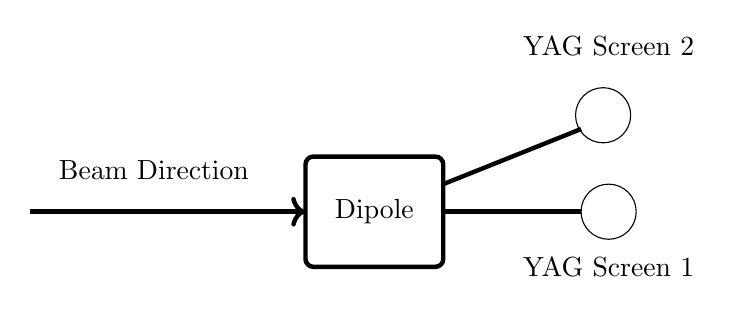
\begin{tikzpicture}[scale=0.7]
			
			\node[] at (2.25,0.75) {Beam Direction};
			\draw[ultra thick, ->] (0,0) -- (5.0, 0.0);
			
			\draw[fill=white, ultra thick, rounded corners =0.1cm] (5.0,1.0)rectangle  
			(7.5,-1.0) node[pos=0.5, align=center] {Dipole};
			
			\draw[ultra thick] (7.5, 0.0) -- (10.0, 0.0);
			\draw[ultra thick] (7.5, 0.5) -- (10.0, 1.5);
						
			\node[] at (10.5, 3) {YAG Screen 2};
			\draw (10.4,1.75) circle (0.5cm);
			
			\node[] at (10.5, -1.0) {YAG Screen 1};
			\draw (10.5,0) circle (0.5cm);
			
		\end{tikzpicture}
	\end{center} 
	\caption{Spectrometer set up in all cases at AWA.}
	\label{fig:spectrometer}
\end{figure*}

\Subsection{Energy Measurement Procedure}
Taking an energy measurement requires a beam trajectory
that is centered through the \lsnote{preceding quadrupole magnets \sout{dipole}}. Otherwise, the beam 
may experience \lsnote{unintentional steering from the quadrupole magnets, and possibly} excessive non-uniform fields 
if it enters the dipole off-axis. The centering is \lsnote{checked by powering \sout{done with} the} two 
quads before the dipole. The center is found by focusing 
in the x-direction, and then the y-direction. If the beam \lsnote{centroid} 
moves \lsnote{horizontally or vertically \sout{to the left or the right}} as it is being focused, 
the quad is "steering", \lsnote{because \sout{and}} the beam is entering the magnets off-axis.
Once the beam is centered through the quads on YAG screen 1, 
the dipole is then turned on to bend the beam.
The two YAG screens are positioned so that when the dipole is off, 
a centered beam will hit YAG screen 1. When the dipole is turned
on, the beam \lsnote{is made to \sout{will}} appear at the center of YAG screen 2 \lsnote{corresponding to a \sout{when the}} 
beam \lsnote{\sout{is}} bent $20^\circ$. In this way, the dipole strength \lsnote{needed to center the beam and YAG screen 2} can 
then be used to determine the beam energy.

\Subsection{Energy Calculation}
Based on the procedure above, there is one number which \lsnote{is used \sout{we use}} to back calculate the mean energy. The \lsnote{\sout{amount of}} current
supplied to the dipole is \lsnote{determined \sout{represented}} by the number of "counts"
keyed into the control system. A counts to current \lsnote{conversion \sout{line}}
is calculated \lsnote{based on \sout{given}} the measurements shown in Table \ref{tab:counts}.  \lsnote{{\it This table reference is not right}}
\begin{table}
\begin{center}
	\caption{Counts to current data for the first dipole in the drive beam line.}
	\begin{tabular}{c c} 
		\toprule
		\toprule
		Counts & Current [A] \\ [0.5ex] 
		\midrule
		1000 & 3.7 \\ 
		
		5000 & 18.8 \\
		
		10000 & 37.5 \\
		
		15000 & 56.3 \\
		\bottomrule
		
	\end{tabular}
\end{center}
\end{table}\label{tab:counts}
Then the B-field is calculated given the current: 
\begin{equation}
	\SI{}{B\,[T]} = (180.9708\cdot \SI{}{I\,[A]} - 7.2053)\cdot 10^{-4}
\end{equation}
There are a few geometric calculations that need to be done using the magnetic field value. 
before we can calculate the energy. 
The radius of curvature, $\rho$, 
can be calculated using the effective length of the dipole, L, and bending angle, $\theta$.
\begin{equation}
	\rho = \frac{L}{2\cdot \sin(\frac{\theta}{2})}
\end{equation}
\lsnote{{\it Starting here, the derivation below is hard to follow.  I am still not sure how you got eq. 2.11.  Then, eq. 2.12 needs more explanation, at least units in the proper places.  Eq. 2.13 seems to be missing a `c' in the momentum term.}}
Using $\rho$, and geometry, we can also estimate the x offset of the
beam after the dipole: 
\begin{equation}
	\Delta x = \rho \left( 1- \cos\theta \right)
\end{equation}
Using this and the famous relationship, $B\rho$ \cite{Wiedemann},
we can relate the B field and the beam momentum. 
\begin{equation}
	\SI{}{p\,\left[\frac{MeV}{c}\right]} = \frac{B\cdot \rho}{3.3356}\cdot 10^3
\end{equation}
We can then calculate the total energy by including the rest mass of the electrons \cite{Griffiths}:
\begin{equation}
	\SI{}{E\,[MeV]} = \sqrt{0.511^2+p^2}
\end{equation}\label{eq:energy}

\Subsubsection{Hard Edge Dipole Example}
\begin{figure*}
	\begin{center}		
		\begin{tikzpicture}[scale=1]
		\node (fig1) at (0,0)
		{\includegraphics[width=0.5\textwidth]{./images/dipole_geometry}};
		\node[fill=white, inner sep=2pt] (txt2) at (-1.25,0.5) {$\frac{L}{2}$};
		\node[fill=white, inner sep=2pt] (txt2) at (-0.5,-2) {$\frac{\theta_k}{2}$};
		\node[fill=white, inner sep=2pt] (txt2) at (0.7,-2) {$\frac{\theta_k}{2}$};
		\node[fill=white, inner sep=2pt] (txt2) at (1.25,0.5) {$\frac{L}{2}$};
		\node[fill=white, inner sep=2pt] (txt2) at (2.5,-2) {$\rho$};
		\end{tikzpicture}
	\end{center} 
	\caption{Simplified drawing of the beam trajectory through a dipole with a uniform field. }
\end{figure*}\label{fig:dipole-geometry}
\lsnote{{\it I do think a numerical example is appropriate here}}
\nrnote{this example is more of a double check and reference for me than for the reader...}
Since this calculation is used several time throughout the 
beam line for different magnets, lets consider a hard edge 
dipole, to show how the above equations can be used to determine
the x offset after the magnet, and the beam energy. 

Let's define the dipole length, $L=\SI{0.2}{[m]}$, angle, $\theta=\SI{20}{degrees}$. 
The corresponding radius is $\rho = \SI{0.5759}{[m]}$. With these values we can now 
calculate the offset, $\Delta x \approx \SI{34}{[mm]}$, which is confirmed by OPAL. 

\nrnote{not sure if I want to include energy since it depends on measured counts....}
Given a count of  energy of $\SI{64.8}{[MeV]}$ given measured counts of 

%%%%%%%%%%%%%%%%%%%%%%%%%%%%%%%%%%%%%%%%%%%%%%%%%%%%%%%%%%%%%%%%%%%%%%%%%%%%%%%%
%%%%%%%%%%%%%%%%%%%%%%%%%%%%%%%%%%%%%%%%%%%%%%%%%%%%%%%%%%%%%%%%%%%%%%%%%%%%%%%%
\Section{Transverse Beam Size Measurements} \label{sec:beamsize}
%%%%%%%%%%%%%%%%%%%%%%%%%%%%%%%%%%%%%%%%%%%%%%%%%%%%%%%%%%%%%%%%%%%%%%%%%%%%%%%%
%%%%%%%%%%%%%%%%%%%%%%%%%%%%%%%%%%%%%%%%%%%%%%%%%%%%%%%%%%%%%%%%%%%%%%%%%%%%%%%%

\lsnote{Intro - why beam size measurements needed?}
Beam size measurements are taken by using YAG screens at multiple z locations along the beam line.
The code used to produce all the following images can be found at this git repository: \lsnote{put url on same line of text}

\url{https://github.com/nneveu/imageProcessing}

\Subsection{Capturing Images}
\nrnote{Add tikz picture here to show how camera is pointed into beam line with mirrors}\\
\lsnote{include some actual YAG images}

\Subsection{Post Processing Images}
A python script was written to take beam images and convert them to profiles in the x and y direction.
This is done in a series of steps, and requires that one or more images can be used as a 
background image and fiducial image. A background image must capture any dark current 
that is present when the beam is not hitting the YAG screen. The fiducial image must 
clearly show the edges of the YAG screen so that a mm/pixel conversion can be calculated.
The following steps detail the post processing from raw image to transverse beam size estimate.

\Subsubsection{Step 1: Calculating the fiducial}

\Subsubsection{Step 2: Remove background intensity}

\Subsubsection{Step 3: Calculate x and y beam profile}

\Subsubsection{Step 4: Fit profile to calculate beam size}


\Section{Bunch Length Measurements}

Must have line break here.\\
\lsnote{Intro: why needed?}

\Subsection{Measurement Technique}
In order to measure the bunch length, we performed an autocorrelation scan
of the CTR \lsnote{{\it define CTR}} produced by the electron distribution \cite{Happek, WBarry}.
\lsnote{{\it Also, describe how CTR produced}} In brief, the CTR is transported into a Michelson interferometer (MI)
where it's split and directed into two MI arms with a half-transparent pellicle \cite{PhysRevSTAB.9.082801}. 
The CTR beams are then combined together at the exit of the MI with the variable path difference.
The resulting CTR intensity is registered with a liquid helium cooled IR Labs
bolometer \cite{bolo} as a function of path difference.
The path difference is then converted into time as $\Delta \tau = 2 \Delta x$.
The resulting FWHM bunch duration is determined from the Gaussian fit of 
the interferogram; see Figure~\ref{interferogram}.
\begin{figure}
	\includegraphics[width=1.0\linewidth]{images/THPMF048f1}
	\caption{An example interferogram for Q=30 nC and laser pulse FWHM of 1.5 ps.}
	\label{interferogram}
\end{figure}
To alleviate the effect of charge fluctuations, we recorded 15 bolometer values for each data point.
The values were then averaged and the errorbars were deduced from the data. The data points
outside of the 3$\sigma$ bracket were considered as outliers and discarded. The resulting
interference pattern as a function of time delay in the MI is similar to that presented in Figure~\ref{interferogram}.

\begin{figure*}[hbt]
	\centering
	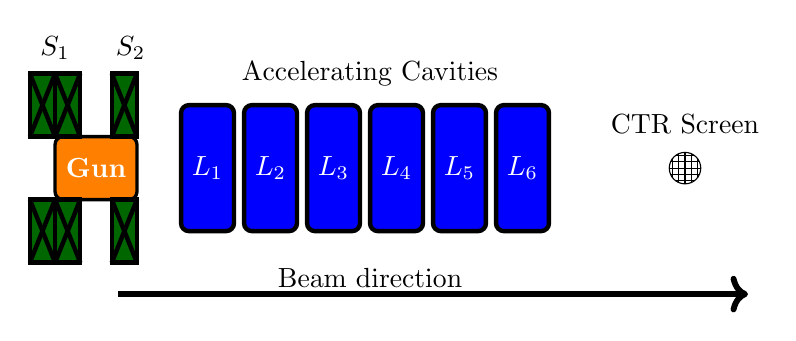
\begin{tikzpicture}[scale=0.8, text=black]
	\def \gunleft {-1.0}
\def \gunright {0.3}
\def \loneright {1.0}
\def \ltworight {2.0}
\def \lthreeright {3.0}
\def \lfourright {4.0}
\def \lfiveright {5.0}
\def \lsixright {6.0}
\def \quadone {7.5}

%Line between kicker and septum
\node[] at (4.0,-0.75) {Beam direction};
\draw[line width=0.75mm, ->] (0.0,-1.0) -- (10,-1.0);

\draw[fill=orange, very thick, rounded corners =0.1cm] (\gunleft,0.5)rectangle (\gunright,1.5) node[pos=.5, white] {\textbf{Gun}} ;
%S1
\node[] at (-1,2.9) {$S_1$};
\draw[ultra thick, fill=black!60!green] (-1.4,-0.5)rectangle  (-1.0,0.5) node[pos=.5, white] {} ;
\draw[black, ultra thick] (-1.4,-0.5) -- (-1.0,0.5);
\draw[black, ultra thick] (-1.4,0.5) -- (-1.0,-0.5);
\draw[ultra thick, fill=black!60!green] (-1.4,1.5)rectangle  (-1.0,2.5) node[pos=.5, white] {} ;
\draw[black, ultra thick] (-1.4,1.5) -- (-1.0,2.5);
\draw[black, ultra thick] (-1.4,2.5) -- (-1.0,1.5);
%S2
\draw[ultra thick, fill=black!60!green] (-1.0,-0.5)rectangle  (-0.6,0.5) node[pos=.5, white] {} ;
\draw[black, ultra thick] (-1.0,-0.5) -- (-0.6,0.5);
\draw[black, ultra thick] (-1.0,0.5) -- (-0.6,-0.5);
\draw[ultra thick, fill=black!60!green] (-1.0,1.5)rectangle  (-0.6,2.5) node[pos=.5, white] {} ;
\draw[black, ultra thick] (-1.0,1.5) -- (-0.6,2.5);
\draw[black, ultra thick] (-1.0,2.5) -- (-0.6,1.5);

%S3
\node[] at (0.2,2.9) {$S_2$};
\draw[ultra thick, fill=black!60!green] (-0.1,-0.5) rectangle  (0.3,0.5) node[pos=.5, white] {};
\draw[black, ultra thick] (-0.1,-0.5) -- (0.3,0.5);
\draw[black, ultra thick] (-0.1,0.5) -- (0.3,-0.5);
\draw[ultra thick, fill=black!60!green] (-0.1,1.5) rectangle  (0.3,2.5) node[pos=.5, white] {};
\draw[black, ultra thick] (-0.1,1.5) -- (0.3,2.5);
\draw[black, ultra thick] (-0.1,2.5) -- (0.3,1.5);
%Linac drawings 
\node[] at (4,2.5) {Accelerating Cavities};
\draw[fill=blue, ultra thick, rounded corners =0.1cm] (\loneright,0)rectangle  ({\loneright+0.84},2) node[pos=.5, white] {$L_1$} ;
\draw[fill=blue, ultra thick, rounded corners =0.1cm] (\ltworight,0)rectangle  ({\ltworight+0.84},2) node[pos=.5, white] {$L_2$};
\draw[fill=blue, ultra thick, rounded corners =0.1cm] (\lthreeright,0)rectangle ({\lthreeright+0.84},2) node[pos=.5, white] {$L_3$};
\draw[fill=blue, ultra thick, rounded corners =0.1cm] (\lfourright,0)rectangle ({\lfourright+0.84},2) node[pos=.5, white] {$L_4$};
\draw[fill=blue, ultra thick, rounded corners =0.1cm] (\lfiveright,0)rectangle ({\lfiveright+0.84},2) node[pos=.5, white] {$L_5$};
\draw[fill=blue, ultra thick, rounded corners =0.1cm] (\lsixright,0)rectangle ({\lsixright+0.84},2) node[pos=.5, white] {$L_6$};

%current optimization point
%\node[draw, fill=yellow, star, star points=5, star point ratio=0.6, minimum size=0.1cm]
%at (12.5,1.0) {$z_1$};
\node[] at (9,1.7) {CTR Screen};
\clip[draw] (9,1) circle (0.25cm);
\draw[step=1mm] (-1,-1) grid (10,10);

%Line between kicker and septum
\draw[very thick] (13.25,0.2) -- (14.5,-0.5);


%Line between septum and dipole
\draw[very thick] (15.6,-0.5) -- (16.5,-0.5);




	\end{tikzpicture}	
	\caption{Beam line layout at the AWA.}
	\label{beamline}
\end{figure*}
\Subsection{Experimental Setup}
The beam line layout is shown in Figure~\ref{beamline}. 
Bunches were allowed to propagate freely to the 
CTR screen. The only focusing elements used were solenoids $S_1$ and
$S_2$. As the bunches passed the CTR screen, light was
emitted through a window located next to the screen, 
as shown in Figure~\ref{bolo}. A slit was used to prevent
background x-rays from reaching the bolometer.
After passing the slit, the CTR propagated to the 
interferometer also shown in Figure~\ref{bolo}.  \lsnote{{\it This section would benefit from a block diagram of the set up}} 
A remotely movable stage inside the interferometer was swept, 
and the resulting combined signal fed to the bolometer. 
%The bolometer was cooled with liquid helium. 
Periodic refilling of the helium \lsnote{is \sout{was}} required \lsnote{when taking data \sout{throughout the day}} in order
to keep the bolometer at \SI{4}{K}. The bolometer sensitivity knob \lsnote{for studies included in this work} was at position ``1'' and
the gain set to 200.
For the case of 1 nC electrons beams, the laser transverse profile was homogenized prior to the vacuum injection \cite{PhysRevAccelBeams.20.103404}.
To produce high-charge 30 nC beams, we implemented an additional laser beamline that bypasses the homogenizer due to the losses in the 
MLA and relay optics.

\begin{figure}
	\centering
	\begin{tikzpicture}[every node/.style={anchor=south west,inner sep=0pt},x=1mm, y=1mm,]   
	\node (fig1) at (0,0)
	{\includegraphics[width=0.5\textwidth]{images/THPMF048f3}};
	\node[fill=white, inner sep=2pt] (txt2) at (35,15) {Interferometer};
	\node[fill=white, inner sep=2pt, rotate=26] (txt2) at (18,19.5) {Slit};	
	\node[fill=white, inner sep=2pt, rotate=20] (txt2) at (13,27) {Window};
	
	\node (fig2) at (0,-50)
	{\includegraphics[width=0.5\textwidth]{images/THPMF048f4}};
	\node[fill=white, inner sep=2pt] (txt2) at (35,-42) {Interferometer};	
	\node[fill=white, inner sep=2pt] (txt2) at (55,-25) {Window};	
	\node[fill=white, inner sep=2pt] (txt2) at (22,-15) {Bolometer};
	\end{tikzpicture}
	\caption{IR labs bolometer and MI interferometer used in the experiment
		to capture CTR light as it exited a window on the beam line. }
	%\label{inter}
	%\caption{Bolometer. }
	\label{bolo}
\end{figure}


\Subsection{Simulations}
\lsnote{{\it This simulation section should be included in next chapter, not here.  The comparison of sim to data and discussion of discrepancies would be important to include there.  The intro type sim stuff is mostly already in sim chapter, so important thing is to have comparison to data added in next chapter.  Here, instead of sim discussion, have modification for independent staging, and previous energy gain measurement.}}
Simulations of the AWA beam line shown in Figure~\ref{beamline}
were performed with the code and OPAL~\cite{opal}.
The gun, accelerating cavities, and solenoids were modeled with 2D
Poisson/Superfish~\cite{fish} files. All field maps were in the T7 format.
Input parameters for the simulations are shown in Table~\ref{simparam}.
Note that on crest refers to the phase of max energy gain.
In the case of the gun, a -~$5^{\circ}$ phase is measured 
w.r.t the peak rf voltage.
\begin{table}[hbt]
	%   \vspace*{-.5\baselineskip}
	\centering
	\caption{Simulation Parameters}
	\begin{tabular}{lcc}
		\toprule
		\toprule
		\textbf{Parameter} & \textbf{Low Charge}  & \textbf{High Charge} \\
		\midrule
		Charge       & 0.3, 0.7, \SI{1.3}{nC}        & \SI{30}{nC}    \\ %[3pt]
		Gun Gradient & \SI{65}{MV/m}     & \SI{65}{MV/m}  \\ %[3pt]
		Gun Phase    & \SI{0}{}$^{\circ}$ & \SI{-5}{}$^{\circ}$ \\		 
		$S_1$        & \SI{230}{A}		 & \SI{500}{A}	  \\
		$S_2$		 & \SI{150}{A}   	 & \SI{235}{A}		 \\
		Linac Phases & On crest          & On crest       \\
		Laser FWHM   & \SI{1.5}{ps}      & \SI{1.5}{ps}   \\ %[3pt]
		Laser Radius & \SI{2}{mm}        & \SI{9}{mm}     \\
		\bottomrule
	\end{tabular}
	\label{simparam}
	%   \vspace*{-\baselineskip}
\end{table}

Four scenarios were simulated, three low charge cases at 0.3, 0.7, and \SI{1}{nC}, and a 
high charge case at \SI{30}{nC}. 
These charges and input parameters were specifically chosen to 
match experimental measurements that had taken place or would 
take place in the future. Each simulation was run with 10,000 particles 
on 8 cores, and ran 2.5 minutes to reach a z location of \SI{17}{m}.
Prior work \cite{benchmark} indicates the bunch length is not 
very sensitive to the number of particles or grid size. 
This would not be the case if we were comparing emittance, or 
transverse characteristics. We expected charge, energy,
and laser parameters to have the most impact on the simulation values.


\Subsection{Results}
Comparison of simulation and experimental results are shown in Figure~\ref{sims}.
\begin{figure*}[!tbh]
	\centering
	\includegraphics[width=0.8\linewidth]{images/THPMF048f5}
	\caption{Comparison of simulations and experimental measurements.}
	\label{sims}
\end{figure*}
While, we do not have an exact match, the results follow the same trends.
The discrepancies indicate there are still adjustments that can be made
to the simulation model. \lsnote{{\it It is not clear what the nature of the problem might be: it could be that some realities of beamline hardware are not included in sim, or as you say, incorrectly matched input parameters.  It would be good to have a discussion on how to narrow down the source of the difference.}} We will continue to try to improve agreement
as more of these measurements are made. 
This can include better measurements of the beam energy and careful attention to other 
beam line parameters such as the laser radius and solenoid strengths.
In the case of high charge simulations, where the agreement is the worst, 
more consideration is needed for large charge fluctuations in the data.\lsnote{{\it <- Not sure what you meant in that last sentence}}

Experimentally measured values of the bunch duration are shown in Table~\ref{exp}.
Note the units in the table are picoseconds and the units in Figure~\ref{sims} are millimeters. \lsnote{{\it So, do the conversion to mm and include in the table.  Then you can have a sentence or two about the comparison.}}
The table gives bunch duration, and the plot gives bunch length for the same data.
We hope these can serve as future reference for others doing experiments at the AWA.
\begin{table}[h]
	\centering
	\caption{Experimental Measurements}
	\begin{tabular}{rcc}
		\toprule
		\toprule
		\textbf{Charge} & \textbf{Bunch Dur. (RMS)} & \textbf{Laser spot size}  \\
		\midrule
		\SI{0.3}{nC} & \SI{2.2}{ps} & 4 mm    \\ %[3pt]
		\SI{0.7}{nC} & \SI{2.6}{ps} & 4 mm   \\ %[3pt]
		\SI{1.3}{nC} & \SI{2.6}{ps} & 4 mm    \\
		\SI{30}{nC}  & \SI{4.1}{ps} & 9 mm \\ %[3pt]
		\bottomrule
	\end{tabular}
	\label{exp}
\end{table}


\lsnote{You need a summary section for the chapter}


%\clearpage

%\include{simulations_optimization}
%\clearpage

\Chapter{Beam Line Design}\label{chp:4}%________________________________


\Section{Introduction}

Independent staging requires two beam lines, with routing of bunch trains via a kicker and septum, 
see Figure \ref{fig:full-staging}. The kicker and septum must direct the beam to a dipole, 
that will straighten the beam trajectory to travel parallel to the original beam path. 
In this configuration the two drive beam lines will be parallel to each other after the dipole.
Several quadrupoles are required to control the beam size, and deliver the desired beam parameters
at the small aperture of the PETS decelerating structure. 
This includes a small transverse size of the beam to allow 100\% transmission, 
and a small bunch length to maximize power extraction from the PETS.
Spectrometer magnets are used to measure the energy of the beam at the end of the beam lines.
This second independent beam line was designed. So far, installation and testing of the kicker has been done.  
The remaining components have been specified, and several are now ready for installation (i.e. septum, quadrupoles, dipoles).
\begin{figure}
		\begin{center}
		\begin{tikzpicture}[scale=\textwidth/35cm, text=black]
		%\begin{tikzpicture}[scale=0.5, text=black]
		\input{./images/full_staging.tex}
		\end{tikzpicture}
	\end{center}
\caption{The arrows indicate what direction the beams travels.
	The guns are located at opposite ends of the bunker and 
	the propagation direction of the beam lines are opposing.
	PETS stands for Power Extraction and Transfer Structure, and ACC stands for Accelerating structure. 
	The subscript on each structure refers to which stage the structures belong to (first or second). 
	The drive line has six accelerating cavities with a maximum beam energy of \SI{70}{MeV}. 
	The witness line has one accelerating cavity with a max beam energy of \SI{15}{MeV}.}
\label{fig:full-staging}
\end{figure}

A kicker design from Indiana University (IU) was used as a base line to design a kicker specific to the
requirements at the AWA. The gap and plate length had to be determined based the beam energy, 
easily or readily available equipment, and mechanical constraints in the AWA tunnel. 
After a design was set, the kicker was fabricated.
Two vacuum tests were performed to verify the fabrication process was successful.
The electronics group at the Advanced Photon Source (APS) provided equipment and helped perform these tests.
The tests included a high voltage (HV) test and Time Domain Reflectometer (TDR) measurement.
Both tests were intended to verify the electrical properties of the kicker were acceptable for operation at HV.
After these tests, the kicker was installed and tested with low and high charge beams. 
The kick was found to be linear with respect to the voltage of the pulser.  
The angle was slightly lower than the simulation result, probably due to reflections at the
connection between the cables and kicker plates. 
The septum design was specified based on simulation work and the kicker angle.
The magnet design was completed at the Institute of Modern Physics (IMP), 
where it was also fabricated. 

The beam line optics also had to be determined and optimized.
The optics include four quadrupoles after the accelerating cavities, 
two quadrupoles on the bent beam line, and three focusing quadrupoles
before the PETS structure.
A point to point matrix calculation was done to ensure that transport of the
beam was possible through the desired kicker gap.  This was followed by an optimization 
performed using the OPAL code and a built-in genetic algorithm. 
There were optimization results in several optics scenarios that can transport 
the beam through the PETS with 100\% transmission.  

This chapter will start with a discussion of the design considerations for the kicker modification for the AWA facility.  
This is followed by a description of the hardware tests done before the kicker installation.  
Simulations relevant to the kicker design will be presented, and compared to beam measurement results.  
The chosen optics design based on the optimization studies will then be presented.


\Section{Kicker Design Theory} \label{theory}

A fast rise time kicker is needed to separate the 
bunch trains supplied by the drive gun.  When the kicker is on, 
bunches passing though it are deflected into an alternate beam line by the kicker field.
The spacing between bunch trains is on the order of nanoseconds; 
it must be long enough to allow the kicker to reach full field before the arrival of the second bunch train, 
and also depends on the layout of the beam lines and laser timing.  
The drive beam and the accelerated `witness' beam must be synchronized so that the 
acceleration field is maximum when the witness beam arrives at the accelerating structure.
Magnetic options for transverse bunch train separation, 
such as a dipole, were disqualified due to their slow rise times 

Borrowing from a successful neighbor, a design implemented by Indiana University (IU) \cite{iukicker}
was adapted to fit the TBA requirements at the AWA. Redesign required consideration
of the length and gap between the kicker plates. Both are key parameters that determine 
what angle the beam will be deflected. Longer plates result in the beam traveling 
in the electromagnetic field for a longer time yielding a larger beam deflection angle). 
A smaller gap increases the field intensity for a given voltage (similar to a parallel plate 
capacitor), increasing the beam deflection angle. 


The kicker is essentially a parallel plate waveguide. 
A $\pm$\SI{30}{kV} power supply can be used to induce a maximum of \SI{60}{kV} potential difference 
across the plates. Each plate will be terminated in a 50 $\Omega$ load.  
The combination of the two plates will result in a static TEM mode 
between the plates. The electric field, $E_x$, and magnetic field, $B_y$,
can be derived from the voltage or current. The electric field, $E_x$, due to a potential, V, is: 
\begin{equation}
E_x=\frac{V}{h}
\end{equation}

where h is the gap height. From Maxwell's equations, we know that the electric and magnetic 
field are related by the speed of light, c, in the case of plane and TEM waves \cite{pozar}. 
From this we can find the magnetic field induced between the plates: 
\begin{equation}
B_y=\frac{E_x}{c}
\end{equation}\label{Bv}
The electrons are traveling at nearly the speed of light, $c$, and move through the kicker on a 
trajectory perpendicular to the fields.  Plugging Equation \ref{Bv} into the Lorentz force equation, 
it is shown that the force exerted on a charge, q, 
from the electric and magnetic fields of the TEM mode are equal. 
\begin{equation}
F=q\,(E_x+v\times B_y)
\end{equation}
\begin{equation}
	F = q \,\left(E_x+c\times \frac{E_x}{c}\right)
\end{equation}

Since the force due to the electric field is equal and oriented in the same direction as the force due to the magnetic field, 
the total kick is twice that from either field alone.  
The angle induced by electric and magnetic fields has been calculated in \cite{iukicker, Wiedemann}
and is rewritten in the following terms:  
\begin{equation}
\theta_E= \frac{V\,L}{h\,T}
\end{equation}
\begin{equation}
\theta_B= \frac{B\,L}{B\rho}
\end{equation}
Where L is the plate length, and T is the kinetic energy of the beam. 
Rigidity, or $B\rho$, is a common accelerator physics term that can be found in text such as Wiedemann \cite{Wiedemann}. 
It is a convenient way to relate the magnetic field and trajectory of an energetic beam traveling through that field.
\begin{equation}
	B\rho=3.33564\,\,T\, \text{[GeV-Tesla]}
\end{equation} 
For a constant magnetic field, as the beam energy increases, the angle decreases. 
The beam is considered "rigid" at higher energies, 
and requires stronger magnetic fields to achieve the same angle, or bending radius ($\rho$).

Using the definitions above, the total angle provided by the kicker is then: 
\begin{equation}
\theta_k = \theta_{total}= \theta_E+\theta_B=2\theta_E=2\theta_B
\end{equation}
We can also calculate the expected deflection, or x offset after the kicker 
using geometry in Figure~\ref{fig:kicker-geometry}, and the expected angle of deflection. 
\begin{figure*}
	\begin{center}		
		\centering
		\begin{tikzpicture}[scale=0.7]
		\node (fig1) at (0,0)
		{\includegraphics[width=0.75\textwidth]{./images/xoffset_geometry}};
		\node[fill=white, inner sep=2pt] (txt2) at (-2.25,7.5) {L};
		\node[fill=white, inner sep=2pt] (txt2) at (-5,-4.5) {$\theta_k$};
		\node[fill=white, inner sep=2pt] (txt2) at (-6.5,5.5) {$\Delta x$};
		\node[fill=white, inner sep=2pt] (txt2) at (-6.5,0) {$x$};
		\node[fill=white, inner sep=2pt] (txt2) at (-2,3) {Beam Direction};
		\node[fill=white, inner sep=2pt] (txt2) at (-1.5,-2) {$\rho$};
		\node[fill=white, inner sep=2pt] (txt2) at (2,2) {$\theta_k$};
		\end{tikzpicture}
	\end{center} 
	\caption{Simplified drawing of beam trajectory through the kicker.
	Where L is the length of the kicker, $\Delta x$ is the beam offset at the exit of the kicker, 
	$\rho$ is the bending radius, and $\theta_k$ is the kicker angle. }
	\label{fig:kicker-geometry}
\end{figure*}
\begin{equation}
\rho = \Delta x + x 
\end{equation}
\begin{equation}
	\Delta x = \rho - \rho \cos \theta_k
\end{equation}
\begin{equation}
	\triangle x = \left(1-\cos\left(\theta_{k}\right)\right)\rho
\end{equation}
Where $\rho$, is the bending radius, $\Delta x$ is the beam offset at the exit of the kicker, 
and $\theta_{k}$ was is the total angle provided by the kicker. 

From these equations, we relate the design parameters gap height, length of the plates, and 
the kinetic energy of the beam. Next, further beam line considerations were included 
to narrow down what angle the kicker needed to supply. 
The largest drive beam energy achievable at the AWA is 65 MeV. 
Therefore the kinetic energy of the beam, T, was set as a constant.
Next mechanical constraints were considered. The two drive beam lines need to be separated
by at least \SI{0.5}{m} so that magnets (quadrupoles and dipoles) can fit on each 
beam line without competing for transverse space. 
\begin{figure*}
		\begin{center}		
		\begin{tikzpicture}[scale=0.7]
		\node (fig1) at (0,0)
		{\includegraphics[width=1\textwidth]{./images/tba_geometry}};
		\node[fill=white, inner sep=2pt] (txt2) at (-5,1.3) {$\theta_k$};
		\node[fill=white, inner sep=2pt] (txt2) at (0.2,0.3) {$\theta_s$};
		\node[fill=white, inner sep=2pt] (txt2) at (5,2.5) {Beam Direction};
		\node[fill=white, inner sep=2pt] (txt2) at (5.2,0) {0.5 m};
		\node[fill=white, inner sep=2pt] (txt2) at (2,-1.5) {$\theta_d$};
		\end{tikzpicture}
		\end{center} 
	\caption{Simplified drawing of the TBA layout. 
			The angle provided by the kicker, $\theta_k$, plus the angle provided by the septum, $\theta_s$,
		    must be less than or equal to $20^\circ$.
			The two beam lines must also be at least \SI{0.5}{m} apart.}\label{fig:triangle}
\end{figure*}

Using geometry as shown in Figure \ref{fig:triangle}, an upper limit on the 
combined kicker and septum angle ($\theta_k+\theta_s$) is based on the existing dipoles at the AWA.
The maximum dipole bend angle, $\theta_d$, is $20^\circ$. 
Therefore, $\theta_{total}$  must be less than $20^\circ$. 
That way the bent beam line can be straightened out using a standard dipole, 
which is readily available at the AWA. 
It is also safer to design away from the limit of the equipment. 
Therefore a bend angle less than $20^\circ$ is preferred and allows room for tolerance errors. 
This has the added benefit of reducing energy spread. 
If the beam is bent at a smaller angle, less coherent synchrotron radiation (CSR) and energy spread will be induced.

Using the equations from Section \ref{theory}, 
tables were made for different plate lengths giving possible gap, angle, and x offset values for comparison. 
The maximum beam energy was used, \SI{75}{MeV}, and the expected pulsar voltage was used, \SI{35}{kV}.
A kicker lengths of \SI{0.42}{m}, \SI{0.5}{m}, and \SI{0.6}{m} were investigated.
From these calculations, the range of possible kicker angles fell between \SI{1}{^\circ} and \SI{3}{^\circ}.
The longest kicker plate option was investigated further with the understanding that 
a larger kicker angle would shorten the drift distance between the kicker and septum, 
and the results for this configuration are shown in Table \ref{tab:kickparam}.
A shorter drift would mean less divergence in the beam before it reaches the next focusing optic (quadrupole).
\begin{table}%[hbt]
	%   \vspace*{-.5\baselineskip}
	\begin{center}
		\caption{Possible kicker parameters for a \SI{75}{MeV} beam,  
		a pulsar voltage of $\pm$ \SI{35}{kV}, 
		and kicker plate length of \SI{0.6}{m}.}\label{tab:kickparam}
	\rowcolors{1}{blue!15}{white}   
	\begin{tabular}{ccc}
		\toprule
		\toprule
		%\rowcolor{blue!30} 
		\textbf{Plate Gap [mm]} & \textbf{Angle [deg]}  & \textbf{X Offset [mm]} \\ \hline
		%\midrule
		20 & 3.2   & 16.7    \\ %[3pt]
		25 & 2.57  & 13.4  \\ %[3pt]
		30 & 2.14  & 11.1 \\		 
		35 & 1.83  & 9.6	  \\
		40 & 1.6   & 8.4		 \\
		45 & 1.43  & 7.4      \\
		50 & 1.28  & 6.7   \\ \hline
		%\bottomrule
	\end{tabular}	
	\end{center}
\end{table}

Next simulations were done to give an estimation of the beam size at the entrance and exit of the kicker.
Typical operating conditions at the AWA were used: accelerating cavities on crest, buck focusing at \SI{500}{A}, 
matching solenoid at \SI{255}{A}, and quadrupoles nearly in a 1:2:1 configuration with \SI{1.7}{A} and \SI{-3.3}{A}.
These are not optimized running conditions, which gives a good upper bound for how the beam will behave before tuning.
An angle of \SI{2}{^\circ} was chosen, as a reasonable starting point based on the values in Table \ref{tab:kickparam}. 
\begin{figure}
	\begin{center}		
		\begin{tikzpicture}[scale=0.7]
		\node (fig1) at (0,0)
		{\includegraphics[width=0.5\textwidth]{./images/scatter_kicker_entrance}%
		\includegraphics[width=0.5\textwidth]{./images/scatter_kicker_exit}};
		\node[fill=white, inner sep=2pt] (txt2) at (6,-4) {X [mm]};
		\node[fill=white, inner sep=2pt] (txt2) at (-5,-4) {X [mm]};
		\end{tikzpicture}
	\end{center} 
	\caption{Simulation of the transverse size of a \SI{40}{nC} 
			beam at the entrance and exit of proposed kicker configuration.}
	\label{fig:beamsizekicker}
\end{figure}  
The resulting beam sizes were about \SI{15}{mm} to \SI{19}{mm} as shown in Figure \ref{fig:beamsizekicker}. 
This requires that the kicker gap be comfortably larger than \SI{20}{mm}, 
and have room for the beam centroid deflection that the kicker will cause.
The gap needed to be large enough to allow the full width of the beam to pass through while allowing extra room
for the transverse offset of the beam as it exits the kicker. 

At this point, it was clear the gap needed to be larger than \SI{30}{mm}, due to the beam size at \SI{40}{nC}. 
Around this time, it was also learned that the max pulsar was $\pm$ \SI{30}{kV}, not $\pm$ \SI{35}{kV} as expected. 
These two factors would drive the possible kick angle below \SI{2}{^\circ}, if the kicker plates remained the same length.
The next question was whether to push for a larger angle by elongating the kicker plates, 
or whether plate gap values at \SI{40}{mm} and above were sufficient, see Table \ref{tab:kickparam}.
Additional mechanical constraints between the kicker and septum were considered. 
One beam pipe will connect the two and the deflected and undeflected 
beams must travel in the same pipe until reaching the septum.
After the septum, the two beams will separate into their own beam pipes.
This connection piece before the split, is a custom vacuum chamber designed at 
AWA and ordered from MDC Vacuum Products, by Scott Doran. 
The large chamber requires more vacuum pumping than other areas, 
which could complicate installation if the chamber was too long. 
In this regard, a larger angle from the kicker would help by shortening the pipe length between the kicker and septum.
Therefore, it was decided to elongate the kicker plates to accommodate the larger gap width and still achieve \SI{2}{^\circ}.
 \begin{table}%[h!]
	\begin{center}
		\caption{Mechanical constraints for TBA beam line.}
		\label{tab:mechanical}
		\rowcolors{2}{blue!10}{white}   
		\begin{tabular}{lc}
			\toprule
			\toprule
			%\rowcolor{blue!30} 
			\textbf{Simulation Parameter} 	&  \textbf{Value} \\ 
			\midrule
			Distance between kicker and septum	&  \SI{1}{m} \\
			Distance between deflected/undeflected beam pipe in septum	& \SI{100}{mm} \\
			Distance between parallel drive lines	& \SI{0.5}{m} \\
			Kicker plate 				& 64 MV\\ 
			Linac Voltages 				& 24-25 MV \\
			Kicker Angle				& -2$^\circ$ \\
			Septum Angle				& -15$^\circ$\\ 
			\bottomrule
		\end{tabular}
	\end{center}
\end{table}

After a discussion on fabrication techniques and the mechanical constraints in Table~\ref{tab:mechanical}, 
it was noted that the maximum kicker plate length could be \SI{1}{m}. 
A new table of voltages and angles was calculated. At this plate length, 
a gap width of \SI{40}{mm} provided roughly \SI{2}{^\circ} of kick again. 
This angle would satisfy the one inch pipe inner diameter spacing in the septum as well. 

For a length of \SI{1}{m}, and gap of \SI{40}{mm}, 
several beam energy and angle scenarios were considered.
As a contingency plan, it was important to consider if the 
beam energy could be lowered to still achieve the desired 
angle and x offset required in the beam line. 
With the pulsar being variable between 18 and 30 kV,
several feasible options were calculated using the equations in Section \ref{theory}, 
and are shown in Figures~\ref{fig:kickerangles} and \ref{fig:kickeroffset}
\begin{figure}%[h]
	\begin{center}
		\includegraphics[width=0.65\textwidth]{./images/AngleVsEnergy}
		\caption{Calculated angle of deflection for \SI{1}{m} long 
		kicker with a gap of \SI{40}{mm} for several beam energies. The target angle is $2^\circ$.}
		\label{fig:kickerangles}
	\end{center}
\end{figure}
\begin{figure}%[h]
	\begin{center}
		\includegraphics[width=0.65\textwidth]{./images/XoffsetVsEnergy}
		\caption{Calculated x offset of the beam after traveling
		through the \SI{1}{m} long kicker with a gap of \SI{40}{mm}.
		The target x offset is about \SI{20}{mm}.}
		\label{fig:kickeroffset}
	\end{center}
\end{figure}
As a double check on the first order calculations in Figures \ref{fig:kickerangles} and \ref{fig:kickeroffset}, 
a PIC simulation was done to estimate the beam 
trajectory in the kicker and septum. 
This work includes rf cavities and space charge effects.
The two estimates match within reason, see Figure \ref{fig:beamtraj}. 
\begin{figure}
	\begin{center}
		\includegraphics[width=0.65\textwidth]{./images/tba_trajectory}
		\caption{Simulation of the transverse offset of a \SI{65}{MeV} beam as 
			it travels through the proposed TBA beam line. 
			Beam is traveling right to left in this simulation. 
			Notice the x offset at the exit of the kicker (\SI{17.5}{m}), 
			is nearly \SI{20}{mm} as predicted in Figure \ref{fig:kickeroffset}.}
		\label{fig:beamtraj}
	\end{center}
\end{figure}

\Section{Preliminary Kicker Tests}

After the design of the kicker was finalized, fabrication began at ANL.
The copper plates and ceramic brackets were fabricated on site at the ANL shops.
High voltage (HV) feedthroughs and cables were purchased from FID GmbH. 
In order to test that the fabrication of the kicker was sound, members of the 
Advanced Photon Source (APS) electronics groups graciously helped perform an 
out of vacuum AC high voltage test. Afterwards they also helped perform and 
analyze a Time Domain Reflectometer (TDR) measurement of the kicker plates
to determine the impedance along the kicker plates, feedthroughs, and cables. 
\begin{figure*}
	\begin{center}		
		\begin{tikzpicture}[scale=0.7]
		\node (fig1) at (0,0)
		{\includegraphics[width=1\textwidth]{./images/kicker}};
		\node[fill=white, inner sep=2pt] (txt2) at (-10,0) {Port 1};
		\node[fill=white, inner sep=2pt] (txt2) at (-5, -5) {Port 3};
		\node[fill=white, inner sep=2pt] (txt2) at (5.5,6) {Port 2};
		\node[fill=white, inner sep=2pt] (txt2) at (10,1) {Port 4};
		\end{tikzpicture}
	\end{center} 
	\caption{CAD drawing of AWA kicker design, courtesy of Scott Doran from AWA.
	Ports are connected the HV cables purchased from FID GmbH. 
	Power is suppled by a puslar also fabricated by FID GmbH and borrowed from the APS Electronics group.}
\end{figure*}\label{fig:AWAkicker}
\begin{figure}%[h]
	\begin{center}
		\includegraphics[width=0.5\textwidth]{./images/FID_feedthrough1}\includegraphics[width=0.5\textwidth]{./images/FID_feedthrough2}
		\caption{High voltage feedthrough purchased from FID GmbH. Left, connection to the HV cables.
		Right, the in vacuum pin that connects to the copper kicker plates.
	Photos supplied by FID GmBH.}
		\label{fig:feedthroughs}
	\end{center}
\end{figure}
\begin{figure}
	\centering
	\includegraphics[width=0.75\textwidth]{./images/kicker_plates}
	\caption{Inside of kicker vacuum chamber after assembly. }
	\label{fig:kicker-plates}
\end{figure}

\Subsection{High Voltage Kicker Test}
Two HV tests were performed at the APS. This was done to ensure the electrical connection 
between the feedthroughs and kicker plates were free of shorts. 
The first test consisted of HV applied in increments to ports 3 and 4 on the kicker.  
Ports 1 and 2 were shorted to ground. There was no leakage current up to \SI{8}{kV} RMS.
The second test reversed the set up with 3 and 4 grounded and ports 1 and 2 exposed. 
There was no leakage current up to \SI{9}{kV} RMS, which was the maximum voltage of the test equipment.
Figure~\ref{fig:AWAHVkicker} shows the connection and location of the kicker in the APS Faraday cage.
\begin{figure}%[h]
	\begin{center}
		\includegraphics[width=\textwidth]{./images/kicker1}
		\caption{High voltage test cage at the APS. 
			The kicker was grounded on one side and exposed to high voltage AC power on the other. 
			The Faraday cage was closed during testing. }
		\label{fig:AWAHVkicker}
	\end{center}
\end{figure}


\Subsection{Time Domain Reflectometer Test}
After the HV test was completed, a Time Domain Reflectometer (TDR) measurement was preformed at the APS~\cite{TDR}, 
with the help of C. Y. Yao, A. Brill, X. Sun and C. Jing.
This technique measures reflections along a conductor and gives information about discontinuities in the line being measured. 
This information was used to determine the impedance along the cables, feedthroughs, and plates of the kicker. 
Ideally, the response would be \SI{50}{\ohm} to reduce reflections and resulting power loss. 
The measurements, plotted by C.Y. Yao in Figure \ref{fig:TDR}, show a larger impedance at the feedthrough locations.
Due to resource and time constraints, it was a goal to use off the shelf parts where possible in fabrication of the kicker.
Therefore, the feedthrough mismatch is expected because they were not specifically designed to couple to the plate geometry.
A substantial amount of time and resources were spent to minimize reflections for the APS kickers plotted in Figure \ref{fig:TDR}.
However, that kicker still deviates from \SI{50}{\ohm} near the feedthroughs.
Given this comparison to the kickers fabricated at the APS, C. Y. Yao advised the mismatch we observed was not dangerous to 
the pulsar or cables that would drive the kicker.  
The only negative result is the reduced amount of voltage supplied to the plates, and therefore, a reduction in the kick given to the beam.
	\begin{figure}
		\begin{center}
			\includegraphics[width=0.75\textwidth]{./images/TDR_AWA_kicker}
			
			(a) TDR single mode measurements of the AWA kicker.
		\end{center}
		\begin{center}
		\includegraphics[width=0.75\textwidth]{./images/TDR_APS_kicker}
	
		(b) TDR single mode measurements of an APS kicker.
		\caption{TDR measurements of the impedance of AWA and APS kickers, plotted by C. Y. Yao.
		Single mode refers to the orientation of the measurement. 
		Only one port of the kicker is driven and measured at a time. }\label{fig:TDR}		
		\end{center}
	
	\end{figure}


\Section{Measurement of Beam Deflection}

Once the kicker was installed, measurements were done to verify it worked as designed with beam.  
The voltage was scanned to check for linearity of the beam offset with voltage.  
The beam size and angle of deflection were measured and compared to simulation results.  
Details of the set up, and results of the studies follow.

The kicker was installed in the AWA drive beam line approximately \SI{16.5}{m} downstream of the cathode.
The HV pulsar was located on the roof of the bunker.
During the beam tests the accelerator was operated in TBA-like conditions based on simulations 
done to optimize for future TBA runs.
The charge was \SI{30}{nC}, the buck focusing solenoid was at \SI{550}{A}, the matching solenoid was at \SI{200}{A}, 
and quadrupoles 5, 6, and 7 were either \SI{-1.53}{A} and \SI{3.08}{A} in a nearly 1:2:1 configuration.
All accelerating cavities were operated at \SI{-20}{^\circ} off crest to minimize energy spread.
The centroid of the beam was calculated for several kicker voltages, and a linear fit was performed.
The R value for the fit in Figure \ref{fig:linear} is 0.99704. This suggests that the beam offset 
is fairly linear with respect to kicker voltage. 
\begin{figure}
	\centering
	\includegraphics[width=0.75\textwidth]{./images/kicker_linearity}
	\caption{Measured deflection of beam due to kicker at several voltages.}
	\label{fig:linear}
\end{figure}

Using the x offset numbers found in Figure~\ref{fig:linear}, 
we can compare the measured angle vs. first order approximations from Section~\ref{theory}.
\begin{figure}
	\centering
	\includegraphics[width=0.75\textwidth]{./images/kicker_angle_comparison}
	\caption{Measured angle provided by the kicker at several voltages.
	These are compared to 1st order calculations for 
	\SI{75}{MeV} and \SI{65}{MeV} beams.
	Smaller angles are expected in the data due to the reflections
	seen at the feedthroughs in TDR measurements, see Figure~\ref{fig:TDR}.}
	\label{fig:angles}
\end{figure}
Beam size data was also taken, see Figure \ref{fig:kickerbeamsize}. 
These measurements were used to calculate the total beam size and 
centroid location of the beam. A combination fit was used to extract 
the beam sizes as described in Section~\ref{sec:beamsize}. 
A Gaussian fit was used for the beam core, and linear fits were used for the tails.
\begin{figure}
	\includegraphics[width=0.5\textwidth]{./images/yag6_kicker_voltage0}%
	\includegraphics[width=0.5\textwidth]{./images/yag6_kicker_voltage18}\\
	\includegraphics[width=0.5\textwidth]{./images/yag6_kicker_voltage20}%
	\includegraphics[width=0.5\textwidth]{./images/yag6_kicker_voltage22}%
	\caption{Examples of beam size data taken during kicker test. 
		Various kicker voltage settings were used and deflection of the beam was observed.}
	\label{fig:kickerbeamsize}
\end{figure}
While the kicker does slightly increase the beam size in the kicked direction, 
the large discrepancy can not be attributed to the kicker alone.
This is clear when looking at the beam sizes when the kicker is off (voltage = 0). 
The beam is already asymmetric before the kicker is turned on.
This is encouraging, as it can be fixed with better control of the quadrupoles.
\nrnote{Argonne cluster was down the last two days. Should be up tomorrow. 
I will add simulation results to this plot after.}
\begin{figure}
	\centering
	\includegraphics[width=0.75\textwidth]{./images/xybeamsizes_high_charge_kicker_scan}
	\caption{Beam size data during voltage scan. Asymmetry between the x and y beam sizes
		 is present even when the kicker is off at V = 0. This suggests the asymmetry is not
	     caused by the kicker alone. }
\end{figure}




\lsnote{Yes - a comparison of the beam sizes to simulation, and a calculation of the deflection versus predicted deflection.  Also, there is a discrepancy, in figure 4.2 the beam size at kicker exit is smaller, not larger.}
\nrnote{that is expected based on the optics. The beam waist is after the kicker, so while the kicker does increase the transverse 
	divergence of the beam, it's still not enough to overcome the focusing of the quadrupoles upstream.}


\Section{TBA Beam Line}

\nrnote{skip this section, not edited yet}
\nrnote{Notes from call: short discussion of the issues, what are you trying to achieve, where are apertures tight.
	comments on what trying to do with optimization and issues}
\lsnote{So here the optics stuff starts - again you will need a little introduction.  What are the goals, and what are you going to present?}
\lsnote{Where are you going with this?  Before you spend a lot of time on it, what are your goals here?}
A drift: 
\begin{equation}
R_d = 
\begin{bmatrix}
1 & L \\
0 & 1
\end{bmatrix}
\end{equation}

A quad: 
\begin{equation}
R_q = 
\begin{bmatrix}
1 & 0 \\
\pm \frac{1}{f} & 1
\end{bmatrix}
\end{equation}

A dipole:
\begin{equation}
R_s = 
\begin{bmatrix}
a & b \\
c & d
\end{bmatrix}
\end{equation}

To convert from focal length to quadrupole strength we must take into account the 
beam energy as well as the dimensions of the quadrupole. 
\begin{equation}
	\frac{1}{f} = kl 
\end{equation}
Where $l$ is the quadrupole's effective length, and k is the gradient w.r.t 
the beam energy and magnet strength \cite{Wiedemann}:
\begin{equation}
	k = \SI{0.2998}{} \frac{g[\SI{}{T/m}]}{p [\SI{}{GeV/c}]}\label{k}
\end{equation}



 To reduce the number of free parameters quickly without using expensive PIC simulations, 
 the transfer matrix of the beam line was considered. Starting at the end of the linac, 
 we consider the first four quadrupoles before the kicker. All the quadruple strengths (4) and
 distances between the quadrupoles (6) are parameters under consideration. To reduce the number
 of variables from 10 to 4, we use the quadruplet telescope module as described by K. Brown in \cite{brown}.  The transfer matrix R, is reduced to:  
 \begin{equation}
 R_q = R_{d4} \cdot R_{q3} \cdot R_{d3} \cdot R_{q2} \cdot R_{d2} \cdot R_{q1} \cdot R_{d1} = 
 \begin{bmatrix}
 \frac{f_2 f_4}{f_1 f_3} & 0 \\
 0 & \frac{f_1 f_3}{f_2 f_4}	
 \end{bmatrix}\label{kb1}
 \end{equation}

\nrnote{add detail about this matrix comes from and expand matrix to x and y}
Where $f_1 \ldots f_4$ stand for the focal lengths of each quad before the kicker. 
Due to other experiments in the AWA tunnel, 
the first quadrupole was required to be at least $\SI{3}{m}$ away from the exit of the 
last accelerating cavity in the linac. This gives the initial drift length and value
for $f_1$. 

\Subsection{Point to Point Check}
To achieve point to point transport of the beam, we can 
equate $f_1 = f_4$ and $f_2 = f_3$. This reduces Eq. \ref{kb1} to:
 \begin{equation}
R_q =
\begin{bmatrix}
1 & 0 \\
0 & 1	
\end{bmatrix}
\end{equation}
We can further simplify the experimental set up by 
assuming $f_1=f_2$. Given the total distance, D, available for the
quads in the beam line, \SI{3.8}{m}, we can then solve
for the focal length $f_1$: 
\begin{align}
	D = 4f_1 + 4 f_2 = 8f_1 = \SI{3.8}{m} \\
	f_1 = \SI{0.475}{m}
\end{align}
Given an energy of \SI{65}{MeV}, a quadrupole length of \SI{11}{cm}, 
and Eq. \ref{k} we can calculate this configuration would require a 
magnet strength of \SI{4.14}{[T/m]}. This is feasible considering the 
max strength is \SI{9}{[T/m]}.

To determine the effect of this configuration on the beam size and divergence
we compare the sigma matrix before and after the qudrupoles:
\begin{align}
	\sigma_1 = R\cdot \sigma_0 \cdot R^T \\
	= 
	\begin{bmatrix}
	1 & 0 \\
	0 & 1	
	\end{bmatrix}
	\begin{bmatrix}
	1 & 0 \\
	0 & 1	
	\end{bmatrix}
    \begin{bmatrix}
	1 & 0 \\
	0 & 1	
	\end{bmatrix} \\
	=
	\begin{bmatrix}
	1 & 0 \\
	0 & 1	
	\end{bmatrix}
\end{align}


\Section{TBA Beam Line Optics Optimization}
 
With the kicker and septum design set, 
and the basic geometry of the beam line laid out, 
an optimization of the beam line optics was performed.
This was done for two reasons. First, to confirm that solutions 
exist at \SI{40}{nC} where the beam is transmitted 100\% through the PETS structure in the deflected beam line.
Second, from the set of feasible solutions, the optics designs with the smallest bunch lengths should be identified.
These two conditions combined will provide an optics solutions that provides the most power output from the test. 

The built in GA in OPAL was again used for these simulations. 
Several rounds of optimizations were tried and many failed for various reasons, 
which include:
\begin{itemize}
	\item using too many objectives (6+)
	\item including too many design variables (15+)
	\item over constraint of the objective values output from the simulation (upper bound too small at \SI{0.1}{mm} for beam sizes)
	\item using bad hyper parameters
\end{itemize}
and so on. 
All iterations can be found in the following repository:
\begin{center}
	\url{https://github.com/nneveu/awa-tba}
\end{center}
which also houses all plotting and simulation scripts used in this chapter.

One draw back of using a GA, is that many simulation parameters 
must be decided empirically after trial and error.
There is no clear guidance on what type of problem set up will be 
best for unique optimization problems such as the beam dynamics in this case.
Along these lines, hyper parameters were chosen based on four experiments ....
\nrnote{should I just reference paper here... or go into details in paper}


\iffalse
the hyper parameters were chosen by doing four small 
GA runs with various settings, see Table \ref{tab:ex}. 
It is clear that the hyper parameters in ex-2 and ex-3 are evolving slower in 
comparison to ex-1 and ex-4. 
Much help was received from A. Adelmann in preparing and discussing these tests.
\begin{table}%[h!]
	\begin{center}
		\caption{Input Parameters for initial twenty four hour TBA optimization experiments. 
			The gene mutation probability was equal to the mutation probability (not shown) in all four experiments. 
			The max number of individuals per generation was~80.}
		\label{tab:ex}
		\rowcolors{2}{blue!15}{white}   
		\begin{tabular}{|lccc|}
	%\toprule
		\rowcolor{blue!30} 
				& \thead{Gene Mutation\\Probability} & \thead{Recombination\\Probability} & \thead{Number of completed\\generations} \\ \hline
			ex-1 &  0.1  & 0.9  &  96 \\
			ex-2 &  0.3  & 0.7  &  81 \\
			ex-3 &  0.8  & 0.2  &  53 \\
			ex-4 &  0.01 & 0.09 &  95 \\ \hline
		\end{tabular}
	\end{center}
\end{table}
\fi

\Subsection{Optimization Setup}\label{setup}
The most successful optimization problem to date entailed optimizing the 
beam size and energy spread at the fifth quarupole on the drive line.
In other words, the first quadrupole between the septum and kicker.
\nrnote{this helps reduce dispersion...include better explanation of this}
\begin{table}%[h!]
	\begin{center}
		\caption{Input GA Parameters for large scale TBA optimization runs.}
		\label{tab:opt-tba}
		\rowcolors{2}{blue!10}{white}   
		\begin{tabular}{lc}
			\toprule
			\toprule
			%\rowcolor{blue!30} 
			\textbf{Simulation Parameter} 	&  \textbf{Value} \\ 
			\midrule
			{Number of Objectives}			&  5 \\
			Number of Design Variables		&  8 \\
			Number of Constraints			&  2 \\
			{Gene Mutation Probability} 	&  0.01\\ 
			{Recombination Probability} 	&  0.09 \\
			{Maximum  Generations}			&  200 \\
			{Initial  Population Size}		&  656\\ 
			Cores per Simulation 			&  8 \\
			Total number of cores			& 2,624  \\
			\bottomrule
		\end{tabular}
	\end{center}
\end{table}
In code form, these parameters translate to an OPAL input file that 
can be found in Appendix~\ref{opt-tba-code}.
\begin{table}%[h!]
	\begin{center}
		\caption{Non-varing Input Parameters for large scale TBA optimization runs.}
		\label{tab:variables}
		\rowcolors{2}{blue!10}{white}   
		\begin{tabular}{lc}
			\toprule
			\toprule
			%\rowcolor{blue!30} 
			\textbf{Simulation Parameter} 	&  \textbf{Value} \\ 
			\midrule
			Cavity Phases		&  -20$^\circ$ \\
			Laser Radius		& 9 mm \\
			Laser Full Width Half Max	& 10 ps \\
			Gun Voltage 				& 64 MV\\ 
			Linac Voltages 				& 24-25 MV \\
			Kicker Angle				& -2$^\circ$ \\
			Septum Angle				& -15$^\circ$\\ 
			\bottomrule
		\end{tabular}
	\end{center}
\end{table}
The OPAL input file and other files needed to run simulations on the ANL cluster 
can be found in the repository listed above.
Details of how the magnet settings, phases, and element locations defined 
in Table~\ref{tab:variables} are also on the repository.


\Subsection{Optimization Results}
After fourty-eight hours, the optimization run described in Section \ref{setup}
completed and the results were analyzed. 
A Pareto front comparing the trade off between bunch length and energy spread was plotted.
\begin{figure}
	\centering
	\includegraphics[width=0.75\textwidth]{./images/dE_vs_zrms_pareto_front_quads_before_Q5}
	\caption{Simulated Pareto front of energy spread vs. bunch length.
	This data was a result of the simulation setup in Section \ref{setup}.}
\label{fig:tba-pareto}
\end{figure}
From Figure \ref{fig:tba-pareto}, there are not many bunch lengths options.
Only one point is excluded from the plot at about \SI{5}{mm}, a region 
not desirable for TBA. The results in the transverse dimension were
more instructive. As expected the beam sizes in the x dimension are larger 
due to the bending elements. This indicates the x dimension will be the 
limiting factor in areas with tight aperatures such as the PETS.
\begin{figure}
	\centering
	\includegraphics[width=0.75\textwidth]{./images/xy_vs_pxy_pareto_front_quads_before_Q5}
	\caption{Simulated Pareto front of beam size vs. momentum.
		This data was a result of the simulation setup in Section \ref{setup}.}
	\label{fig:tba-paretoxy}
\end{figure}
Note the two curves in Figure~\ref{fig:tba-paretoxy}, may not represent the same 
design variables for a point to point comparison. A Pareto analysis always 
chooses the best points w.r.t the objectives chosen. This guarantees no 
relationship between all objectives. 
For example, the smallest beam size in y, at less than \SI{0.35}{mm} on Figure~\ref{fig:tba-paretoxy}, 
may not have the matching solenoid or quad strengths, as the smallest x position 
at a little over \SI{0.35}{mm}. In other words, the best optics scenario for the x dimension
may or may not be the best optics scenario for the y dimension. 

With this in mind, the Pareto front was re-plotted in Figure~\ref{fig:tba-paretoxonly} 
with one key difference. The y values were forced to coincide with the same 
x value design variables. Now a true point to point comparison is possible in this plot.
We chose the x dimension to be the determining plot, 
due to it's clear limitations in comparison to the y dimensions in Figure~\ref{fig:tba-paretoxy}. 
\nrnote{the sentences above are awkward, not sure how to word this} 
\begin{figure}
	\centering
	\includegraphics[width=0.75\textwidth]{./images/xonly_pareto_front_quads_before_Q5}
	\caption{Simulated Pareto front of beam size vs. momentum.
		Adjusted to force y beam sizes to correspond to same design variables 
		as the x beam sizes.
		This data was a result of the simulation setup in Section \ref{setup}.}
	\label{fig:tba-paretoxonly}
\end{figure}
The momentum variance in Figure~\ref{fig:tba-paretoxonly} is small in comparison to 
the beam size variance. Therefore, design variable values resulting in a smaller 
beam size were give higher priority. Table~\ref{tab:designopt}, shows a summary of 
design variables for the four smallest beam sizes.
\begin{table}%[h!]
	\begin{center}
		\caption{Input Parameters for large scale TBA optimization runs.}
		\label{tab:designopt}
		\rowcolors{2}{blue!10}{white}   
		\begin{tabular}{lcccc}
			\toprule
			\toprule
			%\rowcolor{blue!30} 
			\textbf{Simulation Parameter} 	&  \textbf{Value} \\ 
			\midrule
			{Buck Focusing Solenoid [A]}	&  395   & 357   & 328   & 333  \\
			Matching Solenoid [A]		&  209   & 211   & 211   & 184   \\
			Quadrupole 1 [T-m]			&  1.10  & -0.72 & -0.21 & 4.43  \\ 
			Quadrupole 2 [T-m]			&  -1.88 & 0.20  & 0.37  & -4.29 \\
			Quadrupole 3 [T-m]			&  0.39  & -0.73 & -0.26 & 2.50\\
			Quadrupole 4 [T-m]			&  0.61  & 1.92  & 0.25  & -0.99\\ 
			\bottomrule
		\end{tabular}
	\end{center}
\end{table}
The beam size along the beam line was plotted for these optimized points.
\nrnote{a lot more figures to add here, beam sizes along beam line here}
 


\Section{Chapter Summary}

Several design exercises took place to determine the TBA layout at the AWA. 
A stripline kicker was designed using first principles and simulations. 
It was fabricated and assembled at ANL with some parts purchased from third party vendors.
The kickers ability to maintain high voltage was tested with the help of staff members at the APS.
They also added in performing a Time Domain Reflectometer (TDR) measurement to characterize 
the impedance of the kicker, feedthrough, and cable connections. 
A mismatch at the connection point between the kicker plates and feedthroughs was discovered.
While the mismatch reduces the available voltage between the plates, it is not a danger to 
the equipment or beam. After the two out side vacuum tests, the kicker was installed on 
the AWA drive line. It was tested with \SI{30}{nC} beams. 
The beam deflection and angle due to the kicker were measured and 
compared to first order. 
A septum, which will follow the kicker was fabricated by IMP.

Further design work included determination of the beam line geometry
using mechanical and hardware constraints at the AWA. 
A point to point matrix calculation was done to determine if the 
beam size entering the first quadrupoles could be maintained near the kicker.
Next, a beam line optimization was done using the built in genetic algorithm in OPAL.  
Six design variables and five objectives were used. 
The results are plotted, and confirm the beam line geometer can deliver 
a \SI{40}{nC} beam to the PETS location with 100\% transmission.
Future work includes further optimization of the beam line, 
installation of the septum, quadrupoles, and PETS.


 













\clearpage

%\Chapter{Experimental Results} 
%%%%%%%%%%%%%%%%%%%%%%%%%%%%%%%%%%%%%%%%%%%%%%%%%%%%%%%%%%%%%%%%%%%%%%%%%%%%%%%%%%%%%%%%%%%%
%%%%%%%%%%%%%%%%%%%%%%%%%%%%%%%%%%%%%%%%%%%%%%%%%%%%%%%%%%%%%%%%%%%%%%%%%%%%%%%%%%%%%%%%%%%%
\Section{Measurement of Single Stage Power Extraction}
%%%%%%%%%%%%%%%%%%%%%%%%%%%%%%%%%%%%%%%%%%%%%%%%%%%%%%%%%%%%%%%%%%%%%%%%%%%%%%%%%%%%%%%%%%%%
%%%%%%%%%%%%%%%%%%%%%%%%%%%%%%%%%%%%%%%%%%%%%%%%%%%%%%%%%%%%%%%%%%%%%%%%%%%%%%%%%%%%%%%%%%%%
%\Section{Measurement of Single Stage Accelerating Gradient}
%\Section{Measurement of Staged Two Beam Acceleration}
%\clearpage
%%%%%%%%%%%%%%%%%%%%%%%%%%%%%%%%%%%%%%%%%%%%%
%%%%%%%%%%%%%%%%%%%%%%%%%%%%%%%%%%%%%%%%%%%%%


\footnote{My Footnote} 
\Chapter{CONCLUSION}
%   \input{Conclusion.tex}
You need a Conclusion.tex file

\clearpage


%
% APPENDIX
%
\appendix

\Appendix{How to build OPAL on Bebop at ANL} \label{build}
This set of instructions is tailored to the bebop cluster at ANL. 
Intel compilers and intel-MPI were used to build OPAL and all 
the libraries it is dependent on.
\begin{enumerate}[label=Step \arabic*:]
	\item Load modules 

I purge modules first, this will force an error message if any changes
to the system modules occur.
\begin{lstlisting}
	module purge
	module load intel
	module load intel-mpi 
	module load cmake 
	module load gmp   
	module load mpfr  
	module load mpc   
	module load hdf5   
	module load gsl   
	module load intel-mkl
	module load szip
\end{lstlisting}

    \item Set environment variables for compilers 
 
These variables point to intel compilers. 
\begin{lstlisting}
CC=mpiicc;CXX=mpiicpc;F90=ifort;F77=ifort
export CC CXX F90 F77
\end{lstlisting}

    \item Set enviornment variables for self built libraries.
    
I built these libraries separately because they were not available as 
modules on the cluster. 

\begin{lstlisting}
	export PATH="/blues/gpfs/home/neveu/git/H5hut-2.0.0rc3/build:${PATH}"
	
	export H5HUT_HOME=$HOME/git/H5hut-2.0.0rc3/build_intel
	export H5HUT_PREFIX=$H5HUT_HOME
	export H5HUT_DIR=$H5HUT_HOME
	export H5HUT_INCLUDE_DIR=$H5HUT_HOME/include
	export H5HUT_LIBRARY_DIR=$H5HUT_HOME/lib
	
	export BOOST_HOME=$HOME/git/boost_1_62_0/build/
	export BOOST_DIR=$BOOST_HOME
	export BOOST_PREFIX=$BOOST_HOME
	export BOOST_INCLUDE_DIR=$BOOST_HOME/include
	export BOOST_LIBRARY_DIR=$BOOST_HOME/lib
	export BOOST_ROOT=/home/neveu/git/boost_1_62_0/
	echo $BOOST_ROOT
	echo $BOOST_DIR
\end{lstlisting}

    \item Call cmake 
    
There are two cmake calls I use depending on if I'm building for 
BDW (\verb|-axCORE-AVX2|) or KNL (\verb|-axMIC-AVX512|) architecture. 
    
\begin{lstlisting}
cmake -DCMAKE_INSTALL_PREFIX=/home/neveu/software/opal-1.9/bdw -DCMAKE_CXX_FLAGS="-lsz -axCORE-AVX2" ..
\end{lstlisting}

    \item Call make, then make install
I usually call make with a large number of cores to speed up the compilation.    
\begin{lstlisting}
	make -j 30 
	make install
\end{lstlisting}

\end{enumerate}



%\moretox

\Appendix{OPAL stuff? MCS Stuff?}

Your second appendix text....

\newpage
%
% BIBLIOGRAPHY
%
\bibliographystyle{plain}
\bibliography{thesis}

\end{document}  % end of document





























